

\chapter{Πειραματική Αξιολόγηση}\label{ch:results}
Η πειραματική αξιολόγηση έγινε στην Matlab 7.11.0. Η πηγή τοποθετήθηκε στο κέντρο (0,0) της κυκλικής περιοχής ανάπτυξης των στατικών κόμβων. Για καλύτερα στατιστικά
αποτελέσματα εφαρμόστηκε πολλές φορές η ανάπτυξη των στατικών κόμβων και κάθε πείραμα εκτελέστηκε 100 φορές. Η στατιστική ανάλυση των αποτελεσμάτων δηλώνουν
πολύ μεγάλη συγκέντρωση γύρω από την μέση τιμή, επομένως στα σχεδιαγράμματα φαίνονται μόνο οι μέσες τμές.

Για να αξιολογηθούν σωστά οι στρατηγικές και οι αλγόριθμοι που προτάθηκαν, η πειραματική αξιολόγηση γίνεται κάθε φορά σε 3 τελείως διαφορετικής φύσεως πρωτόκολλα
δρομολόγησης που όμως το καθένα αντιπροσοπεύει την αντίστοιχη οικογένεια πρωτοκόλλων δρομολόγησης. Τα πρωτόκολλα είναι το Greedy \cite{greedy_protocol}, το οποίο
ουσιαστικά αποτελεί ένα πρωτόκολλο σαν το CTP (Collection Tree Protocol) το οποίο έχει μια δενδρική μορφή, το Leach \cite{leach_protocol} το οποίο αποτελεί ένα
ιεραρχικό με συστάδες πρωτόκολλο και το $E_{i}$ \cite{debp_protocol} το οποίο αποτελεί ένα πρωτόκολλο εξισορρόπησης ενέργειας.

Αφού οι $N$ κόμβοι είναι ομοιόμορφα κατανεμημένοι σε μία κυκλική περιοχή $\mathcal{A}$ ακτίνας $R$ εφαρμόστηκε ένα γνωστό κατώφλι συνδεσιμότητας προκειμένου να
μεγιστοποιηθεί η πιθανότητα των γενημένων τυχαίων στιγμιότυπων να είναι συνδεδεμένα. Πιο συγκεκριμένα, αφού $\mathcal{A}\subset \mathbb{R}^2$, ένα στιγμιότυπο του
μοντέλου τυχαίων γεωμετρικά γραφημάτων (random geometric graphs) $\mathcal{G}(\mathcal{X}_N;r)$ κατασκευάζεται ως εξής: επιλέγονται $N$ σημεία $\mathcal{X}_N$
ομοίομορφα τυχαία στο $\mathcal{A}$. Το σύνολο $V = \mathcal{X}_N$  είναι το σύνολο των κορυφών του γράφου και δύο κορυφές συνδέονται αν οι ευκλείδιες αποστάσεις
τους είναι το πολύ $r$. Στα \cite{rg1,rg2} δείχνεται οτι το κατώφλι συνδεσιμότητας για τα $\mathcal{G}(\mathcal{X}_N;r)$ είναι $r_c = \sqrt{\frac{\ln N}{\pi N}}$. Σε
αυτή την εργασία θεωρούνται τυχαία στιγμιότυπα από $\mathcal{G}(\mathcal{X}_N;r)$ με ποικίλη πυκνότητα , επιλέγοντας $r = \sqrt{\frac{c\ln N}{\pi N}}$, για διάφορες
τιμές του $c>1$, το οποίο εγγυάται οτι το παραγόμενο τυχαίο στιγμιότυπο είναι συνδεδεμένο με μεγάλη πιθανότητα. Καθόλη την διάρκεια των πειραμάτων η παράμετρος $c$
είναι σταθερή με μεγαλύτερες τιμές για το Greedy πρωτόκολλο γιατί είναι πιο επιρρεπή σε γρηγορότερες αποσυνδέσεις.

Αφού το δίκτυο είναι αρκετά πυκνό, θεωρείται οτι κάθε μετάδοση κοστίζει $r^{2}$ σε μονάδες ενέργειας, όπου $r$ είναι ακτίνα μετάδοσης ενός κόμβου. Αφού οι κόμβοι
καθώς και η γέννηση γεγονότων είναι ομοιόμορφα κατανεμημένη, η μέση τιμή των βημάτων (hops) που χρειάζονται για ένα γεγονός να ταξιδέψει από τον πρώτο κόμβο που το
ανίχνευσε μέχρι την Πηγή είναι $\frac{R}{2}\cdot \frac{1}{r}$. Επομένως, η μέση ενέργεια που καταναλώθηκε για την δρομολόγηση ενός γεγονότος από τον πρώτο κόμβο μέχρι
την Πηγή είναι $r^2\frac{R}{2r} = \frac{rR}{2}$ και για την συνολική ενέργεια που κανατλώθηκε στο δίκτυο είναι $E_{total} = \frac{\mu r R}{2}$, όπου $\mu$ είναι ο
αριθμός των γεγονότων. Στα πειράματα δώθηκε ενέργεια ίση με $E_{total} = \frac{h\mu r R}{4}$, για $h > 1$ προκειμένου να εξασφαλιστεί οτι οι κόμβοι πεθαίνουν μετά
από αρκετούς γύρους.

Τα πειράματα επικεντρώνονται στις ακόλουθες μετρικές απόδοσης:
\begin{itemize}
\item \textbf{Ζωντανοί κόμβοι κατα την πάροδο του χρόνου}, δηλαδή ο αριθμός των κόμβων που έχουν εναπομείνουσα ενέργεια που τους καθιστά ικανούς να λειτουργούν , κατα
την διάρκεια εκτέλεσης ενός πειράματος
\item \textbf{Συνδεσιμότητα κατατ την πάροδο του χρόνου}, δηλαδή ο μέσος βαθμός (ο μέσος αριθμός γειτόνων) του κάθε κόμβου κατα την διάρκεια εκτέλεσης ενός πειράματος
\item \textbf{Χρονοκάλυψη}, δηλαδή ο μέσος αριθμός κάλυψης (coverage) του δικτύου από κόμβους 1000 τυχαίων σημείων δίκτυο κατα την πάροδο του χρόνου. Στα γραφήματα τα
χρώματα υποδηλώνουν τον αριθμό κάλυψης του σημείου σύμφωνα με την εικόνα \ref{fig:coverage_sample}.
\item \textbf{Ενεργιακός χάρτης του δικτύου}, ο οποίος είναι μια απεικόνιση του συνολικού δικτύου που εμφανίζονται οι σχετικές ενέργειες των κόμβων
\end{itemize}

\begin{figure}[h]
  \centering
  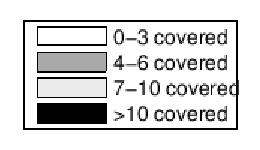
\includegraphics[width=0.3\textwidth]{images/network_coverage.eps}
  \caption{Ο μέσος αριθμός κάλυψης των σημείων σε χρώματα.}
  \label{fig:coverage_sample}
\end{figure}

Στην πειραματική αξιολόγηση ερευνούνται οι στρατηγικές που μελετήθηκαν στο κεφάλαιο \ref{ch:strategies_solution} ώστε να βρεθή η βέλτιστη στρατηγική και οι
αντίστοιχοι παράμετροι ενέργειας στους κόμβους και στον κινητό φορτιστή με κύριο στόχο την μεγιστοποίηση του χρόνου ζωής του δικτύου. Στα 3 πρώτες σειρές πειραμάτων
χρησιμοποιείται ο προσαρμοστικός φορτιστής ο οποίος διασθητικά είναι και ο καλύτερος. Στην τελευταία σειρά πειραμάτων, αφού βρεθούν οι κατάλληλες παράμετροι
κατανομής της ενέργειας για το δίκτυο, ο προσαρμοστικός φορτιστής συγκρίνεται με τους υπόλοιπους φορτιστές.

\section{Με και Χωρίς Φόρτιση}\label{sc:result1}
Η πρώτη σειρά από πειράματα αφορά την σύγκριση του δικτύου με φόρτιση και του δικτύου χωρίς φόρτιση. Όταν επιλέγεται το δίκτυο να είναι χωρίς φόρτιση τότε η συνολική
ενέργεια του δικτύου κατανέμεται όλη στους στατικούς κόμβους του δικτύου, δηλαδή ο κάθε κόμβος ξεκινάει με το 100\% της αρχικής του ενέργειας. Αντίθετα όταν
επιλέγεται το δίκτυο να είναι με φόρτιση, δηλαδή με έναν κινητό φορτιστή που φορτίζει τους κόμβους, η συνολική ενέργεια κατανέμεται ανάμεσα στους στατικούς κόμβους
και τον κινητό φορτιστή. Οι στατικοί κόμβοι σε αυτή την περίπτωση δεν ξεκινάνε με πλήρη αρχική ενέργεια αλλά με ένα ποσοστό της αρχικής ενέργειας. Στο πείραμα αυτό,
καθώς δεν έχει βρεθεί η βέλτιστη αναλογία ενέργειας ανάμεσα στον κινητό φορτιστή και τους στατικούς κόμβους, οι τελευταίοι ξεκινάνε με το με το 60\% της αρχικής τους
ενέργειας και επομένως ο φορτιστής κατέχει αρχικά το 40\% της αρχικής ολικής ενέργειας του δικτύου. Χρησιμοποιείται ο προσαρμοστικός φορτιστής. Τα αποτελέσματα των
πειραμάτων φαίνονται στις εικόνες \ref{fig:1exp_1_1}, \ref{fig:1exp_2_1}, \ref{fig:1exp_3_1}, \ref{fig:1exp_3_2}, \ref{fig:1exp_3_3}, \ref{fig:1exp_4_1},
\ref{fig:1exp_4_2} και \ref{fig:1exp_4_3}. Η διαισθητική εικόνα που αφήνουν τα αποτελέσματα είναι οτι δίνοντας ένα μέρος της συνολικής αρχικής ενέργειας του δικτύου
στον φοτιστή, ακόμα και χωρις να έχει βελτιστοποιηθεί το μέγεθος που δίνεται, υπάρχουν σημαντικά καλύτερα αποτελέσματα σε όλες τις μετρικές.



%%%%%%%%%%%%%%%%%%%%%%%%%%%% 1. LIFETIME %%%%%%%%%%%%%%%%%%%%%%%%%%%%%%%%%%%%%
\begin{figure}[H]
  \centering
  \subfloat[Greedy]{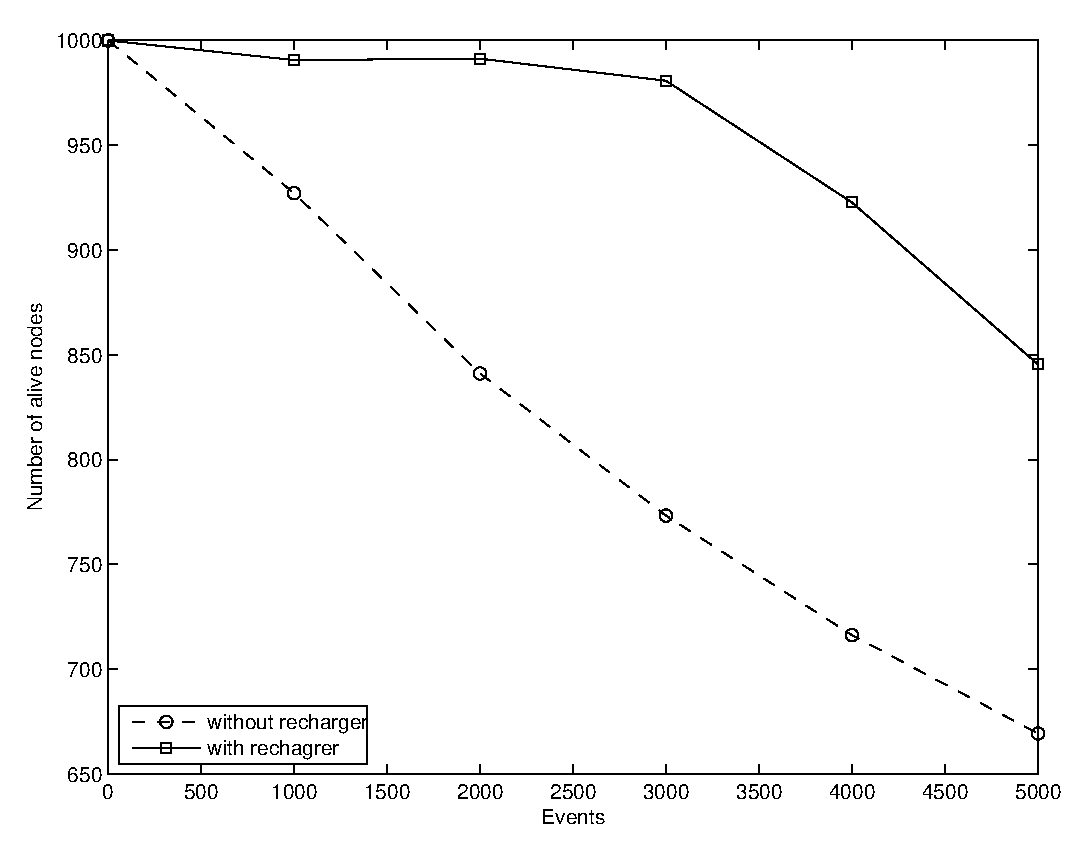
\includegraphics[width=0.32\textwidth]{experiments/classic/1.norechargeVSrecharge/alive_nodes_greedy_nonrc-rc.eps}}
  \subfloat[Leach]{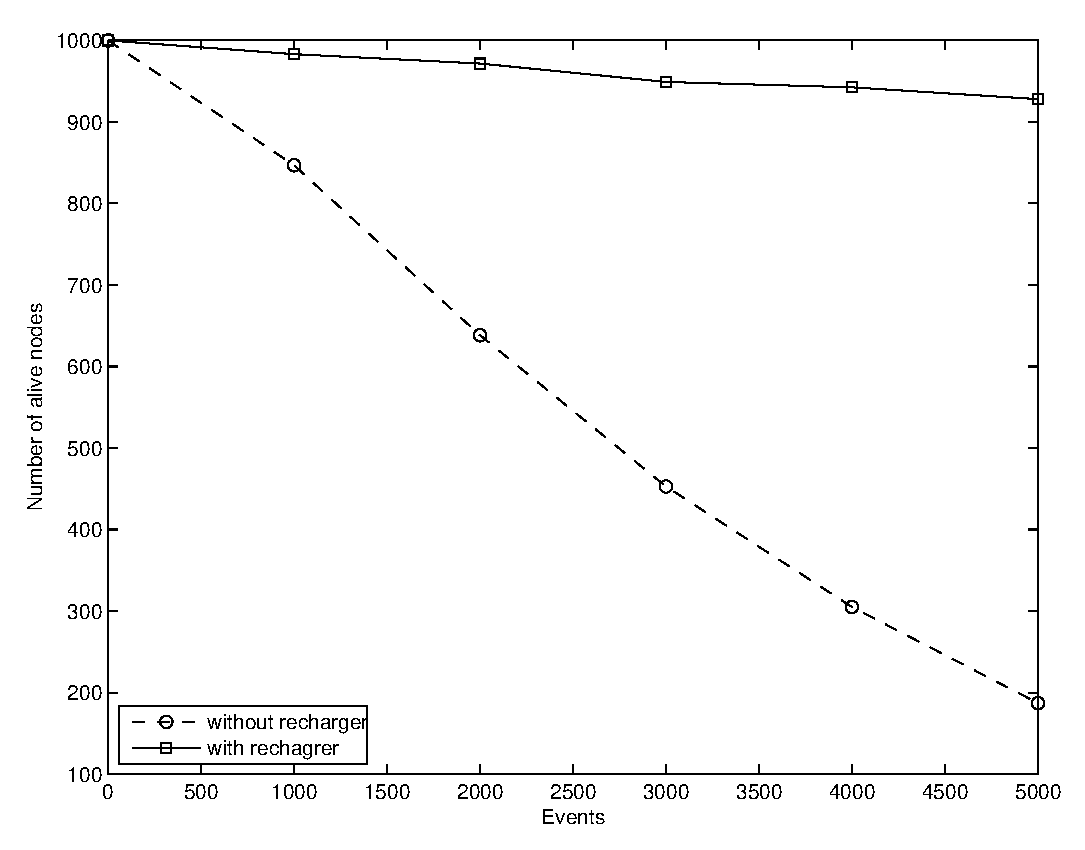
\includegraphics[width=0.32\textwidth]{experiments/classic/1.norechargeVSrecharge/alive_nodes_leach_nonrc-rc.eps}}
  \subfloat[$E_{i}$]{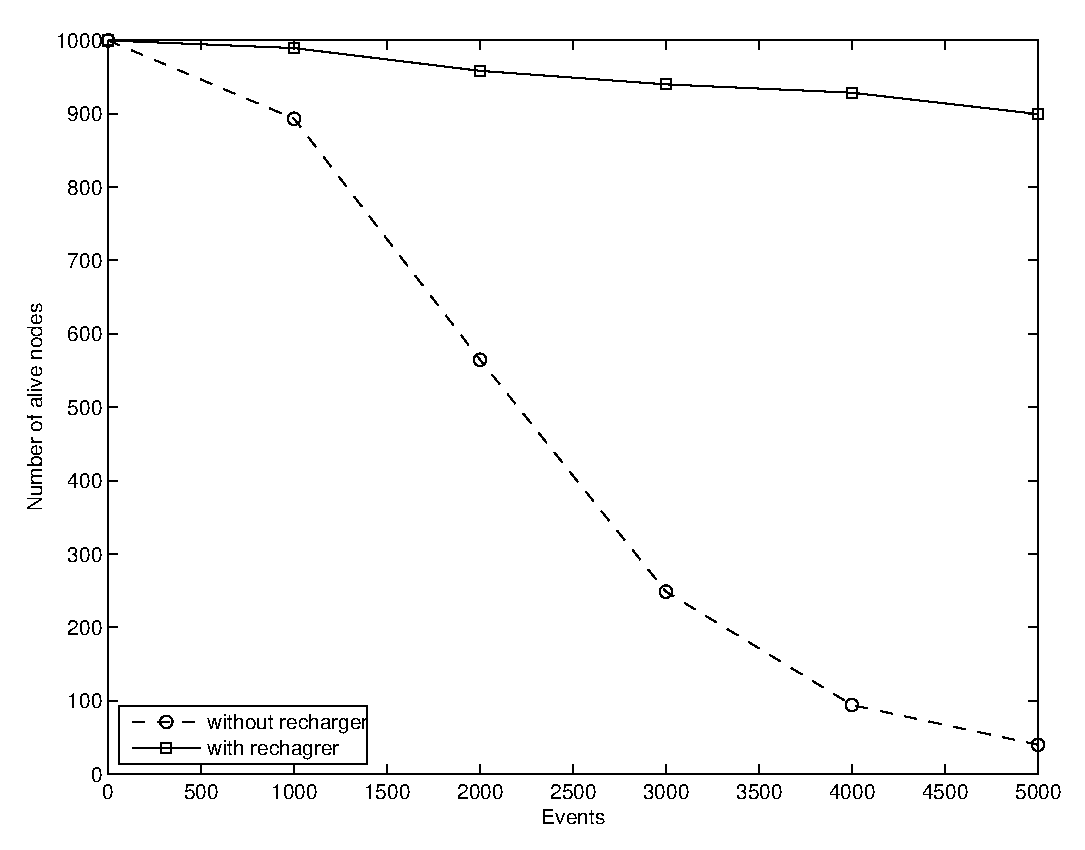
\includegraphics[width=0.32\textwidth]{experiments/classic/1.norechargeVSrecharge/alive_nodes_ei_nonrc-rc.eps}}
  \caption{Ζωντανοί κόμβοι κατά την πάροδο του χρόνου. Η συνεχόμενη γραμμή αντιστοιχεί στο δίκτυο με κινητό φορτιστή. Γίνεται εμφανές οτι υπάρχει αύξηση
	του χρόνου ζωής του δικτύου αν δοθεί μέρος της συνολικής ενέργειας
   στον φορτιστή (εδώ δόθηκε 40\%).}
  \label{fig:1exp_1_1}
\end{figure}

%%%%%%%%%%%%%%%%%%%%%%%%%%%% 2. CONNECTIVITY %%%%%%%%%%%%%%%%%%%%%%%%%%%%%%%%%%%%%
\begin{figure}[H]
  \centering
  \subfloat[Greedy]{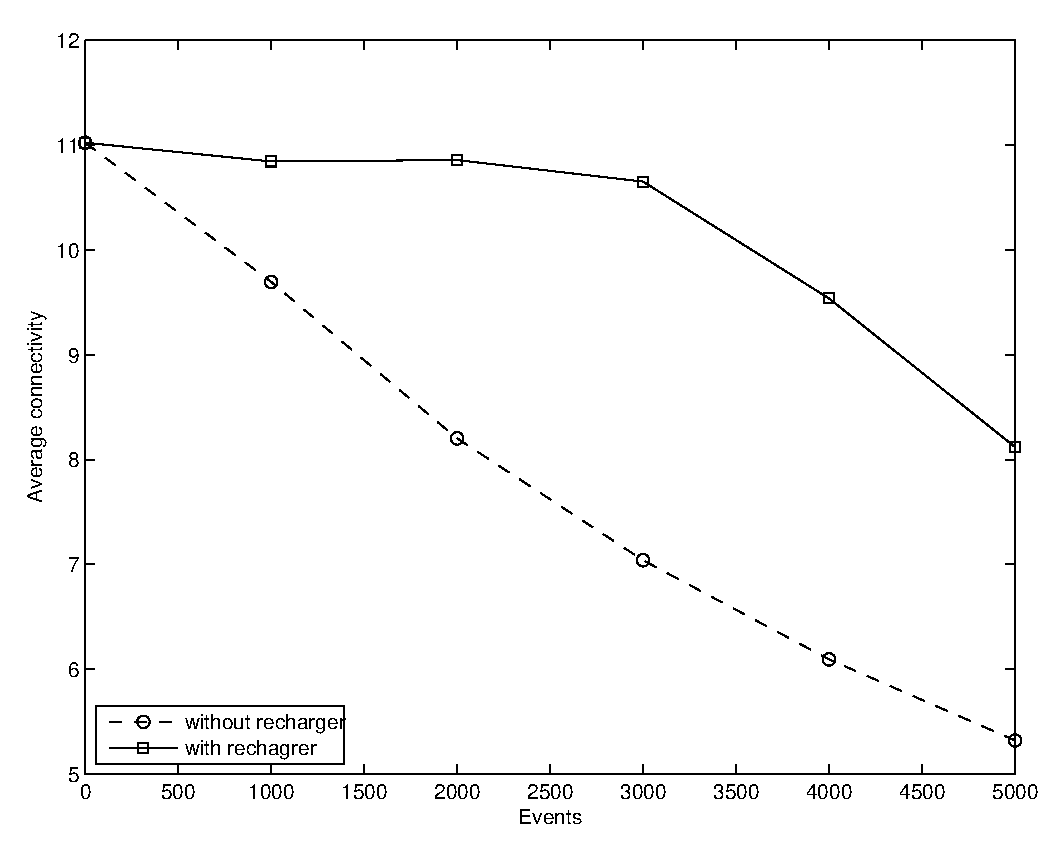
\includegraphics[width=0.32\textwidth]{experiments/classic/1.norechargeVSrecharge/connectivity_greedy_nonrc-rc.eps}}
  \subfloat[Leach]{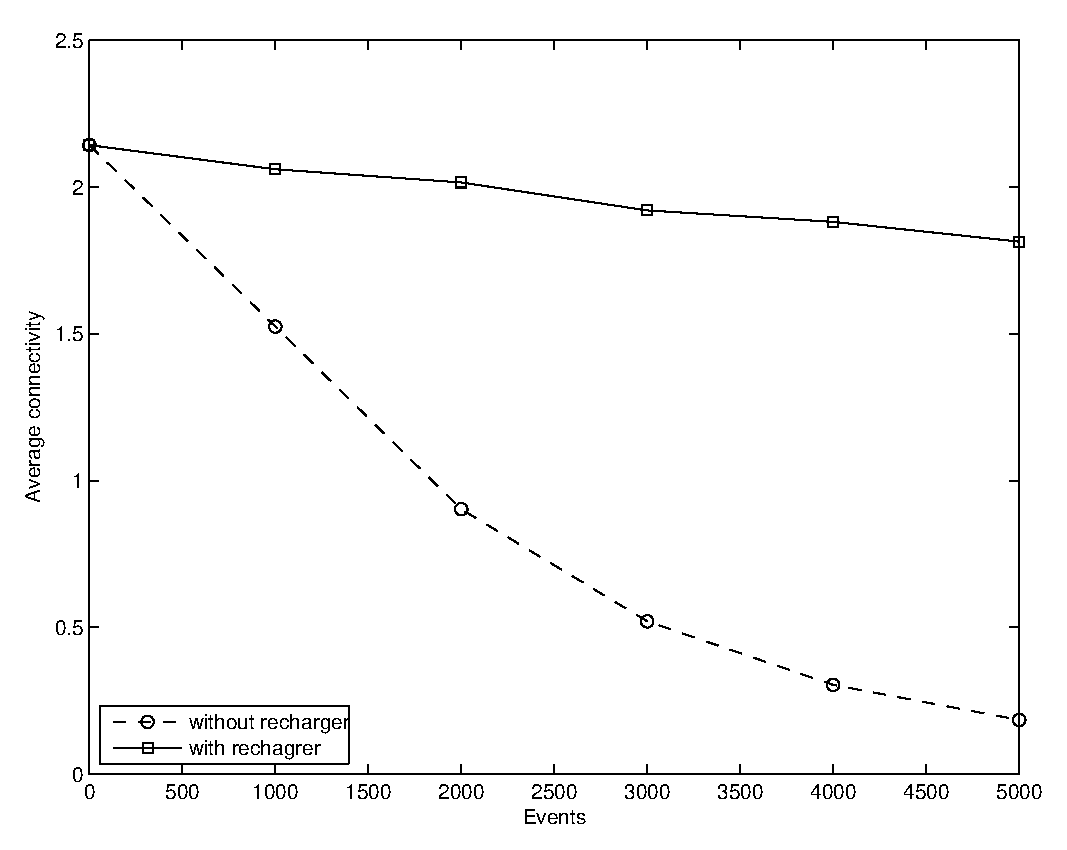
\includegraphics[width=0.32\textwidth]{experiments/classic/1.norechargeVSrecharge/connectivity_leach_nonrc-rc.eps}}
  \subfloat[$E_{i}$]{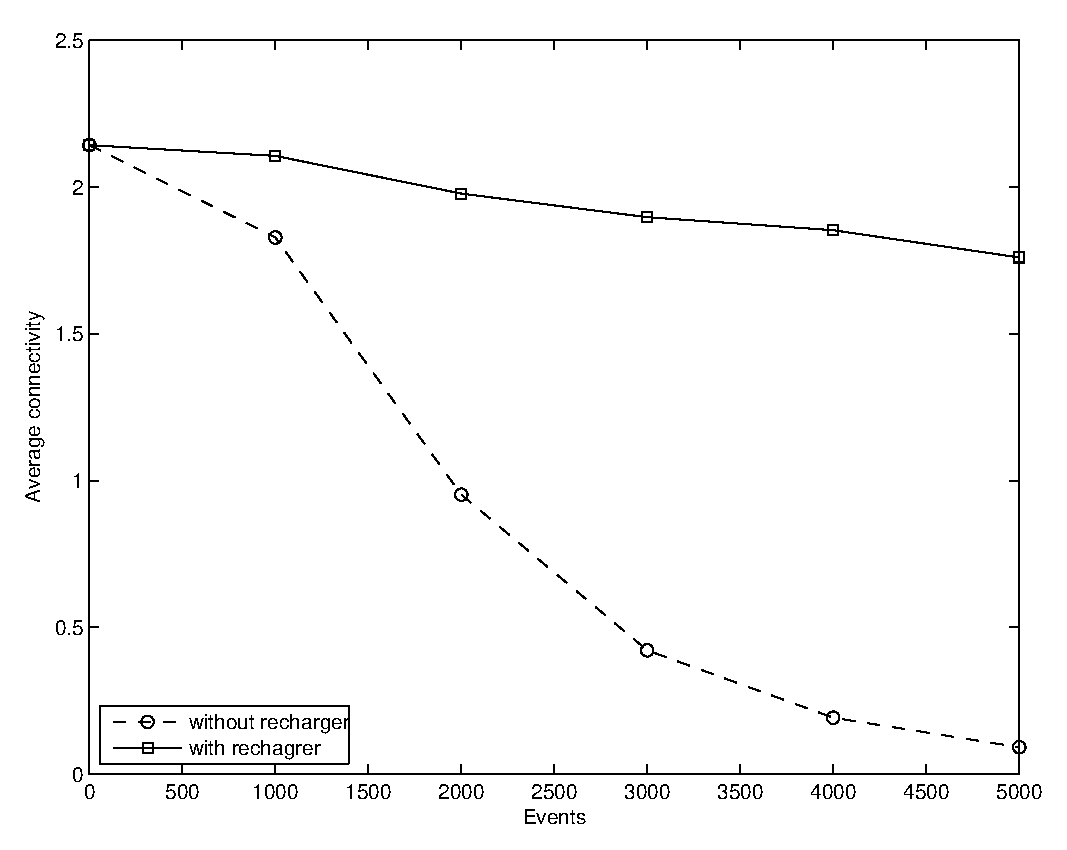
\includegraphics[width=0.32\textwidth]{experiments/classic/1.norechargeVSrecharge/connectivity_ei_nonrc-rc.eps}}
  \caption{Συνδεσιμότητα κατα την πάροδο του χρόνου. Η συνεχόμενη γραμμή αντιστοιχεί στο δίκτυο με κινητό φορτιστή. Υπάρχει σημαντική αύξηση της συνδεσιμότητας του
	δικτύου αν δοθεί μέρος της συνολικής ενέργειας
   στον φορτιστή (εδώ δόθηκε 40\%).}
  \label{fig:1exp_2_1}
\end{figure}


%%%%%%%%%%%%%%%%%%%%%%%%%%%% 3. COVERAGE %%%%%%%%%%%%%%%%%%%%%%%%%%%%%%%%%%%%%

\begin{figure}[H]
  \centering
  \subfloat[Greedy]{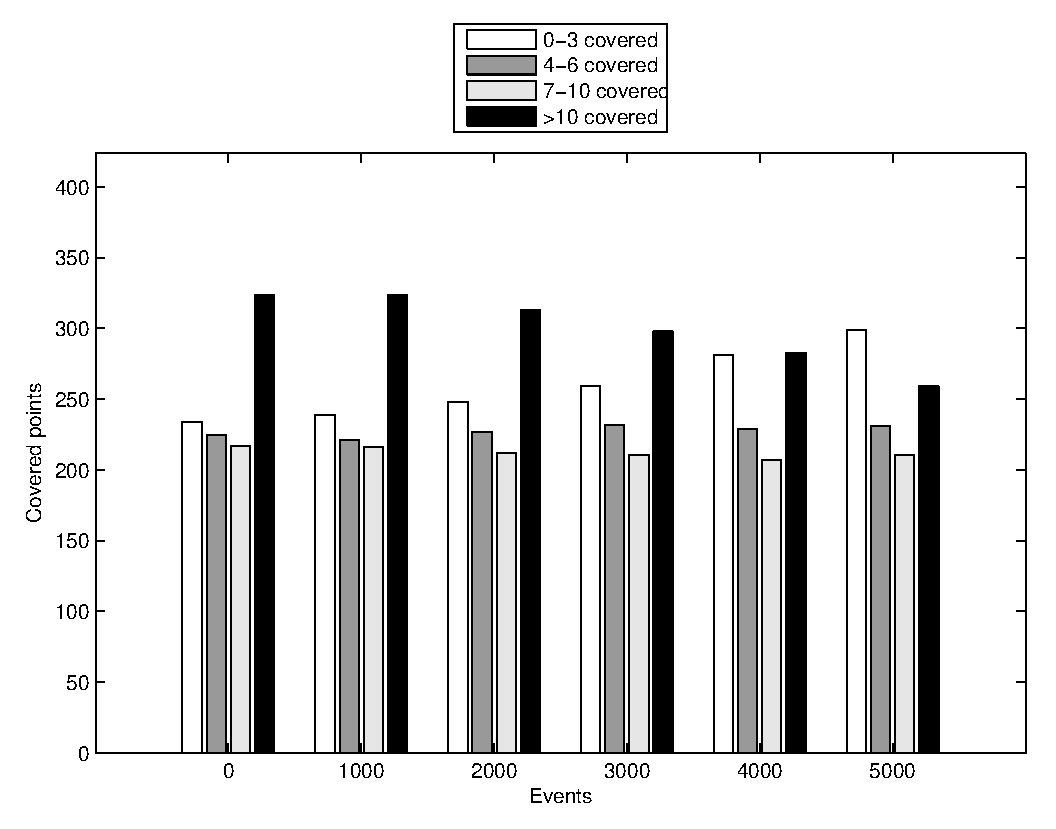
\includegraphics[width=0.48\textwidth]{experiments/classic/1.norechargeVSrecharge/coverage_greedy.eps}}
  \subfloat[Greedy με Φορτιστή]{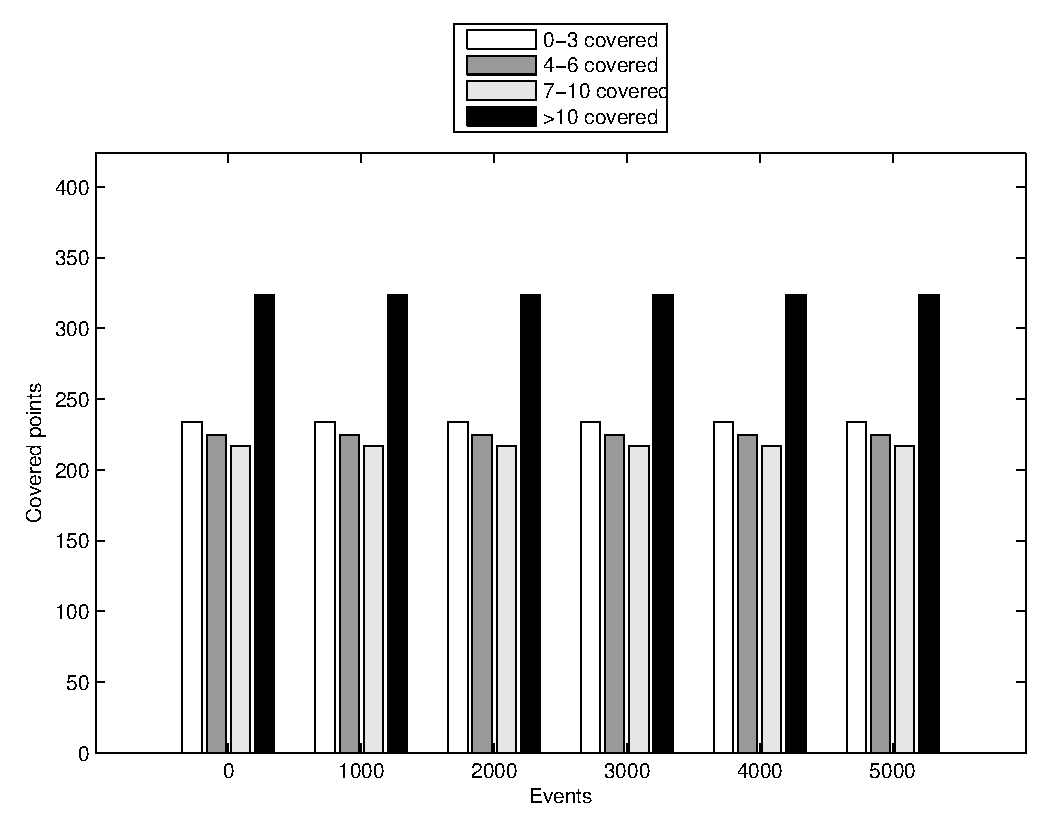
\includegraphics[width=0.48\textwidth]{experiments/classic/1.norechargeVSrecharge/coverage_greedy_rc.eps}}
  \caption{Κάλυψη του δικτύου κατα την πάροδο του χρόνου για το πρωτόκολλο Greedy. Συγκρίνοντας τις 2 γραφικές παραστάσεις φαίνεται οτι στο δίκτυο με φορτιστή
υπάρχει καλύτερη κάλυψη των σημείων του δικτύου.}
  \label{fig:1exp_3_1}
\end{figure}

\begin{figure}[H]
  \centering
  \subfloat[Leach]{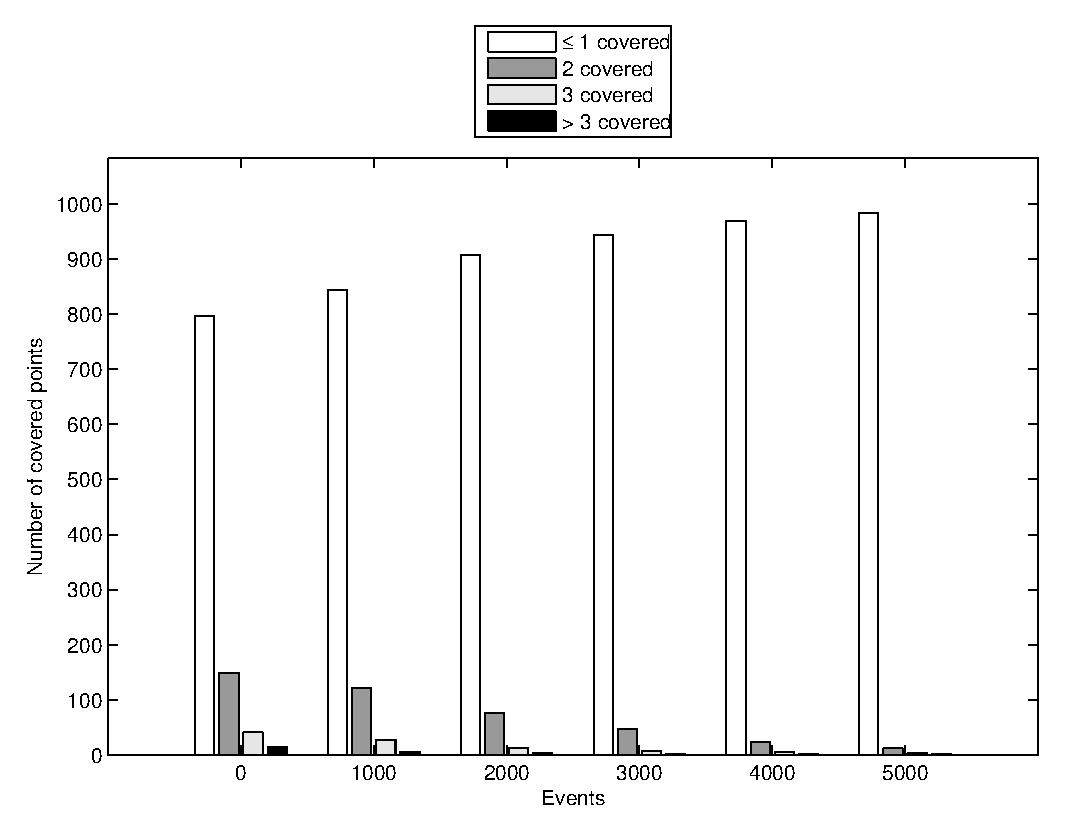
\includegraphics[width=0.48\textwidth]{experiments/classic/1.norechargeVSrecharge/coverage_leach.eps}}
  \subfloat[Leach με Φορτιστή]{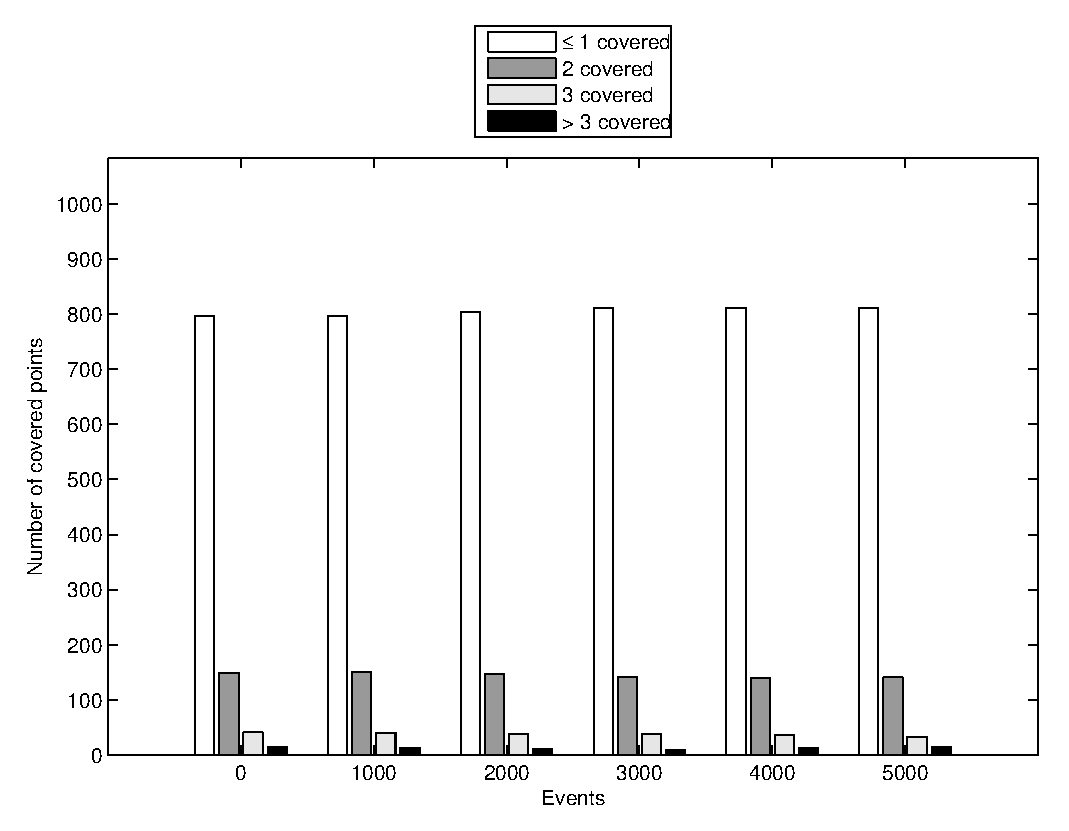
\includegraphics[width=0.48\textwidth]{experiments/classic/1.norechargeVSrecharge/coverage_leach_rc.eps}}
  \caption{Κάλυψη του δικτύου κατα την πάροδο του χρόνου για το πρωτόκολλο Leach. Συγκρίνοντας τις 2 γραφικές παραστάσεις φαίνεται οτι στο δίκτυο με φορτιστή
υπάρχει καλύτερη κάλυψη των σημείων του δικτύου.}
  \label{fig:1exp_3_2}
\end{figure}

\begin{figure}[H]
  \centering
  \subfloat[$\text{E}_{i}$]{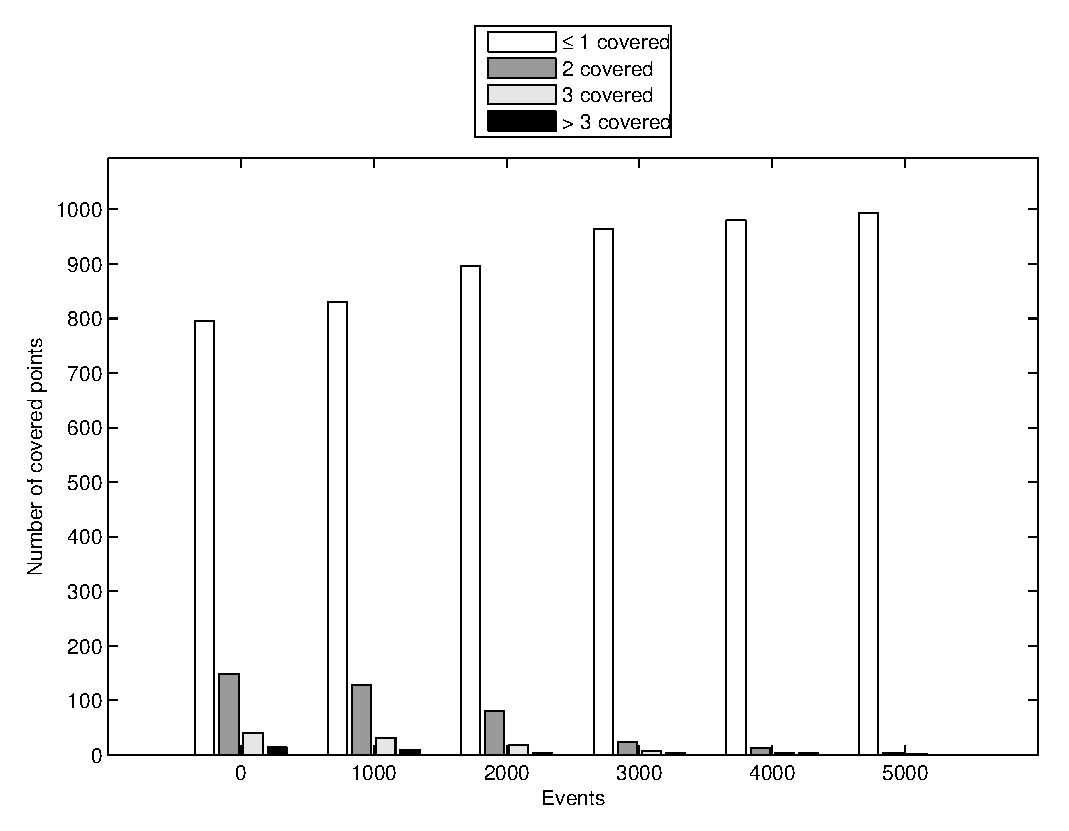
\includegraphics[width=0.48\textwidth]{experiments/classic/1.norechargeVSrecharge/coverage_ei.eps}}
  \subfloat[$\text{E}_{i}$ με Φορτιστή]{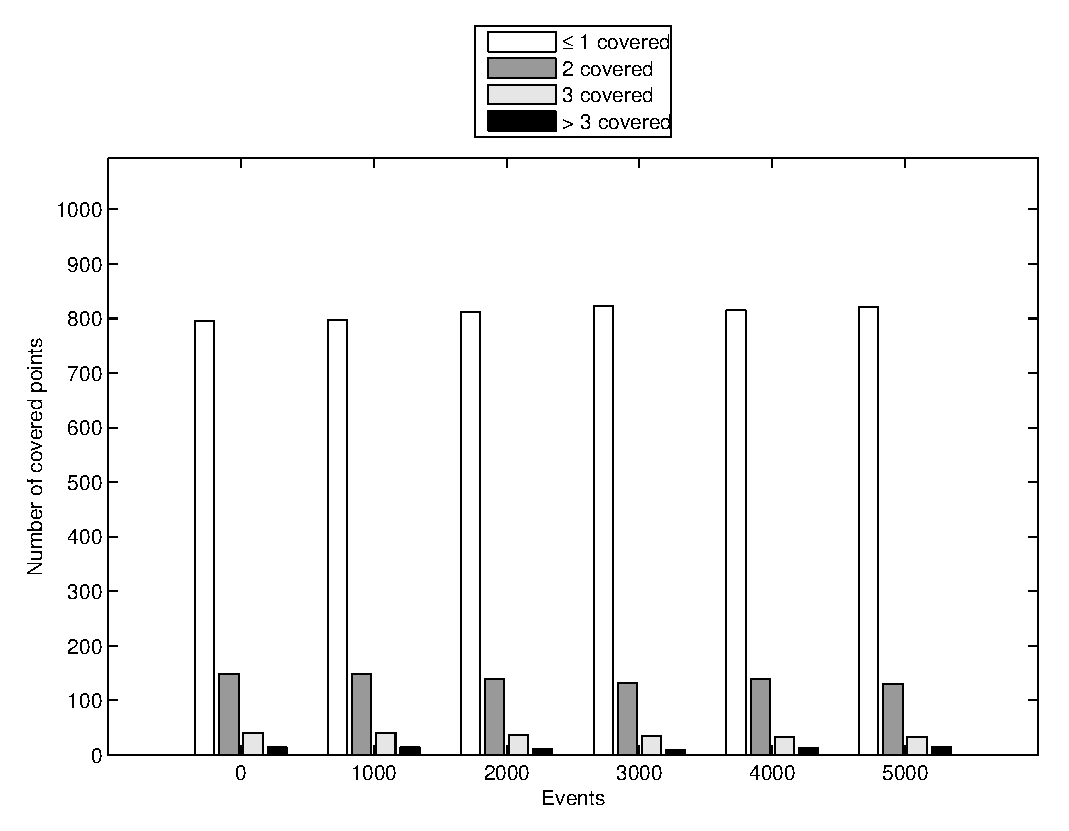
\includegraphics[width=0.48\textwidth]{experiments/classic/1.norechargeVSrecharge/coverage_ei_rc.eps}}
  \caption{Κάλυψη του δικτύου κατα την πάροδο του χρόνου για το πρωτόκολλο $\text{E}_{i}$. Συγκρίνοντας τις 2 γραφικές παραστάσεις φαίνεται οτι στο δίκτυο με φορτιστή
υπάρχει καλύτερη κάλυψη των σημείων του δικτύου.}
  \label{fig:1exp_3_3}
\end{figure}




%%%%%%%%%%%%%%%%%%%%%%%%%%%% 4. ENERGY MAPS %%%%%%%%%%%%%%%%%%%%%%%%%%%%%%%%%%%%%

\begin{figure}[H]
  \centering
  \subfloat[Greedy]{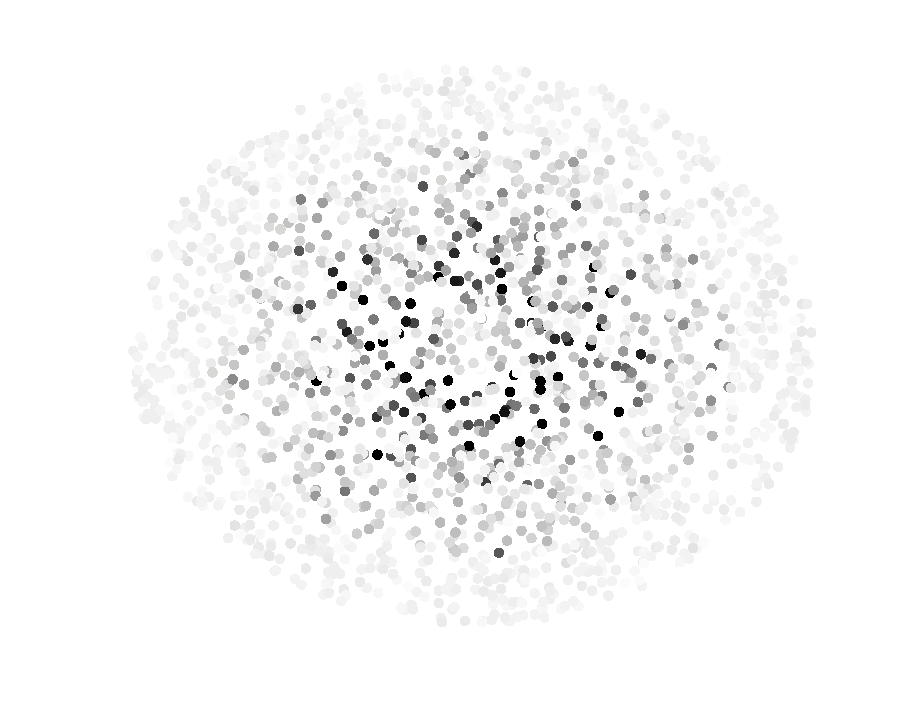
\includegraphics[width=0.48\textwidth]{experiments/classic/1.norechargeVSrecharge/energy_greedy.eps}}
  \subfloat[Greedy με Φορτιστή]{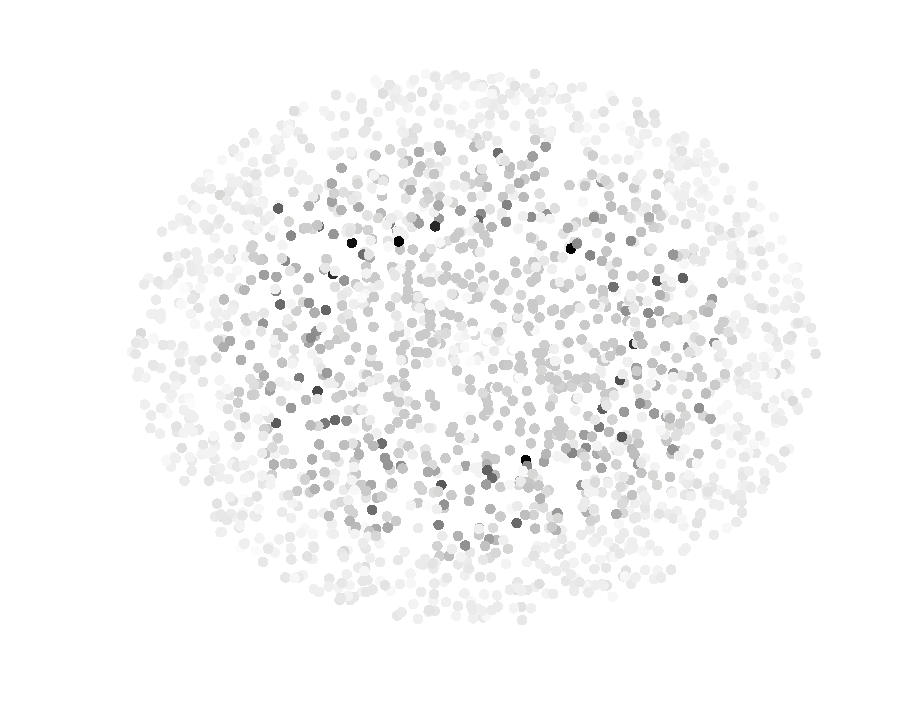
\includegraphics[width=0.48\textwidth]{experiments/classic/1.norechargeVSrecharge/energy_greedy_rc.eps}}
  \caption{Ενεργιακός χάρτης του δικτύου κατα την πάροδο του χρόνου για το πρωτόκολλο Greedy. Όσο πιο μαύρο τόσο λιγότερη ενέργεια έχει ο κόμβος. Συγκρίνοντας τις 2
γραφικές παραστάσεις φαίνεται οτι στο δίκτυο με φορτιστή υπάρχει καλύτερη εξισορρόπηση ενέργειας.}
  \label{fig:1exp_4_1}
\end{figure}

\begin{figure}[H]
  \centering
  \subfloat[Leach]{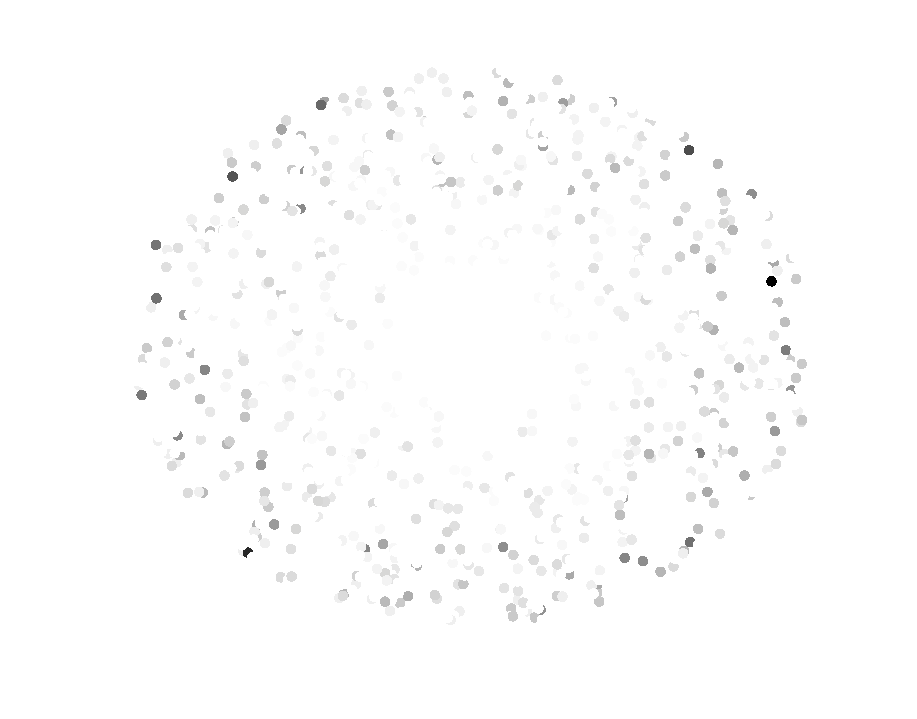
\includegraphics[width=0.48\textwidth]{experiments/classic/1.norechargeVSrecharge/energy_leach.eps}}
  \subfloat[Leach με Φορτιστή]{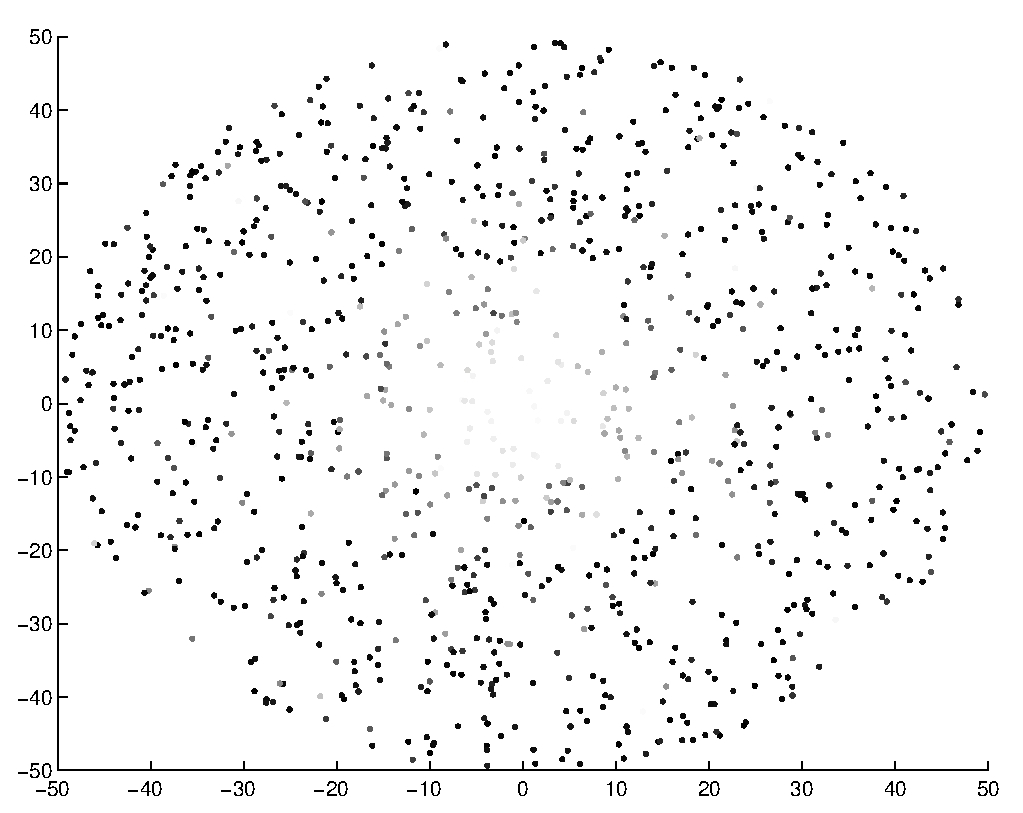
\includegraphics[width=0.48\textwidth]{experiments/classic/1.norechargeVSrecharge/energy_leach_rc.eps}}
  \caption{Κάλυψη του δικτύου κατα την πάροδο του χρόνου για το πρωτόκολλο Leach. Όσο πιο μαύρο τόσο λιγότερη ενέργεια έχει ο κόμβος. Συγκρίνοντας τις 2 γραφικές
παραστάσεις φαίνεται οτι στο δίκτυο με φορτιστή υπάρχει καλύτερη εξισορρόπηση ενέργειας.}
  \label{fig:1exp_4_2}
\end{figure}

\begin{figure}[H]
  \centering
  \subfloat[$\text{E}_{i}$]{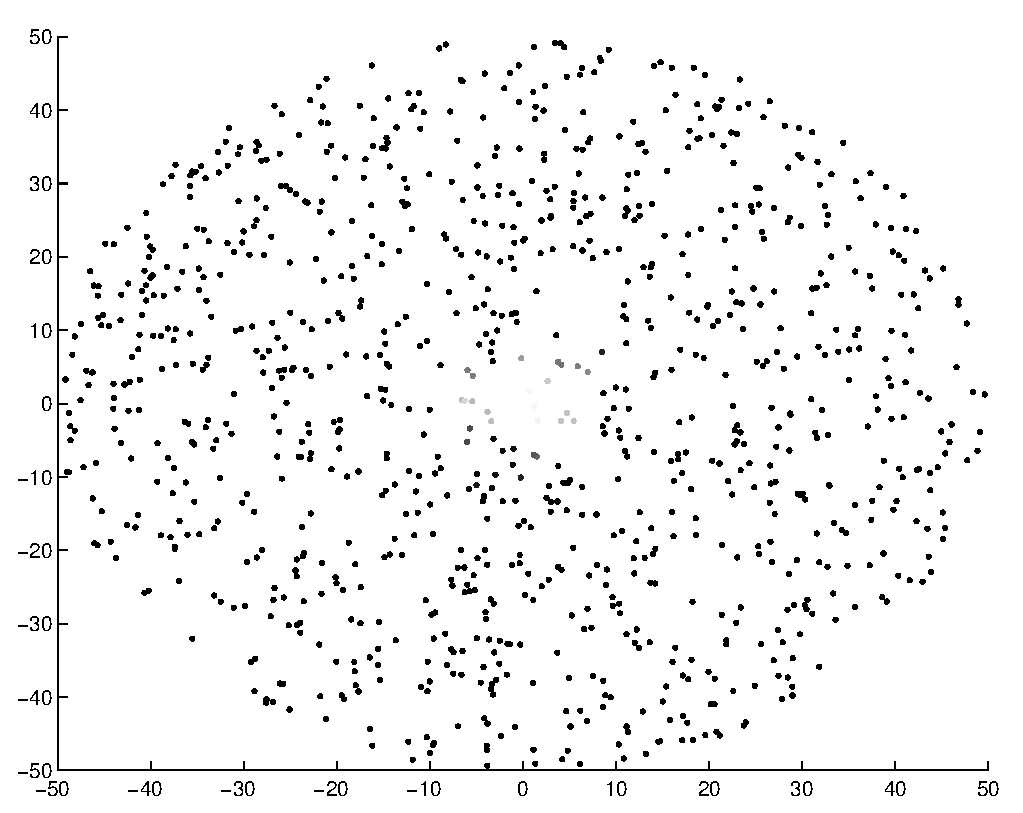
\includegraphics[width=0.48\textwidth]{experiments/classic/1.norechargeVSrecharge/energy_ei.eps}}
  \subfloat[$\text{E}_{i}$ με Φορτιστή]{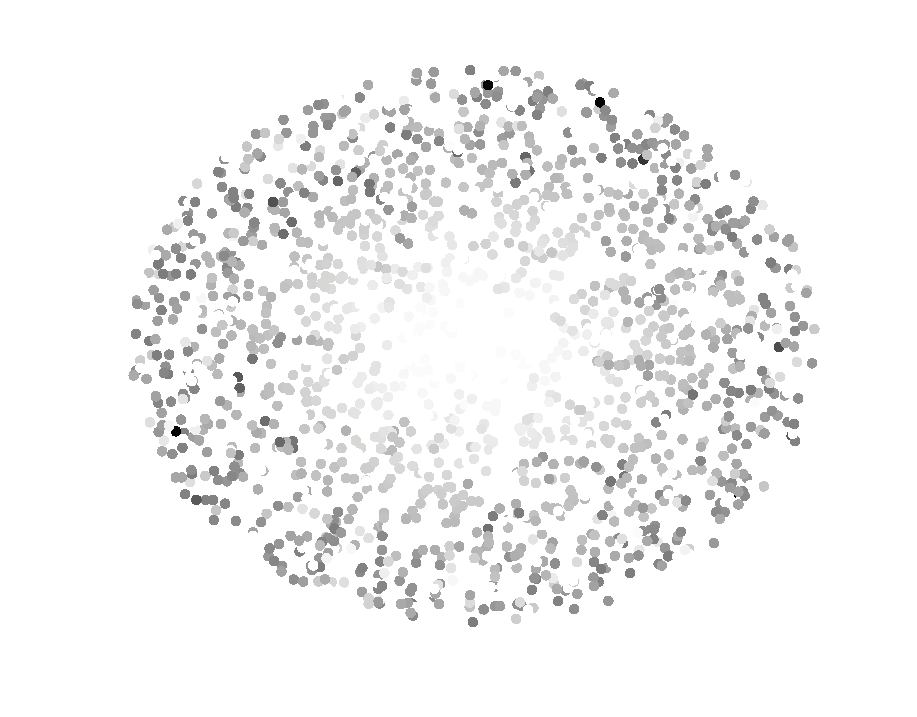
\includegraphics[width=0.48\textwidth]{experiments/classic/1.norechargeVSrecharge/energy_ei_rc.eps}}
  \caption{Κάλυψη του δικτύου κατα την πάροδο του χρόνου για το πρωτόκολλο $\text{E}_{i}$. Όσο πιο μαύρο τόσο λιγότερη ενέργεια έχει ο κόμβος. Συγκρίνοντας τις 2
γραφικές παραστάσεις φαίνεται οτι στο δίκτυο με φορτιστή υπάρχει καλύτερη εξισορρόπηση ενέργειας.}
  \label{fig:1exp_4_3}
\end{figure}

Όπως φαίνεται και από τα σχεδιαγράμματα, στην περίπτωση που στο δίκτυο χρησιμοποιείται φόρτιση, αυτό έχει μεγαλύτερο χρόνο ζωής αφού ο φορτιστής επιλέγει να δώσει
την ενέργεια εκεί που πραγματικά την χρειάζεται.







\section{Ολική και Μερική Φόρτιση}\label{sc:result2}
Η πρώτη παραμετροποίηση ή στρατηγική της διαδικασίας της φόρτισης που μελετάται είναι μέχρι ποιο επίπεδο θα πρέπει ο κινητός φορτιστής να φορτίζει τους στατικούς
κόμβους. Οι 2 στρατηγικές που συγκρίνονται είναι:
\begin{itemize}
  \item \textbf{Oλική φόρτιση}, δηλαδή σε κάθε καινούργια φόρτιση ο φορτιστής φορτίζει μέχρις ότου ο στατικός κόμβος να ανακτήσει πλήρως την αρχική του ενέργεια
  \item \textbf{Μερική φόρτιση}, δηλαδή σε κάθε καινούργια φόρτιση ο φορτίζει μέχρις ότου για την ενέργεια του στατικού κόμβου $e_{i}$ ισχύει οτι
\begin{align*}
e_{i} \approx \frac{E^{curr}_{MC}}{E^{init}_{MC}}\cdot E^{max}_{sensor}
\end{align*}
όπου $E^{curr}_{MC}$, $E^{init}_{MC}$ η τρέχουσα ενέργεια και αρχική ενέργεια του κινητού φορτιστή ενώ $E^{max}_{sensor}$ η αρχική ενέργεια ενός στατικού κόμβου.
\end{itemize}
Ξανά οι στατικοί κόμβοι σε αυτή την περίπτωση δεν ξεκινάνε με πλήρη αρχική ενέργεια αλλά με ένα ποσοστό της αρχικής ενέργειας, και συγκεκριμένα
με το 60\% της αρχικής τους ενέργειας και επομένως ο φορτιστής κατέχει αρχικά το 40\% της αρχικής ολικής ενέργειας του δικτύου. Τα αποστελέσματα των πειραμάτων
φαίνονται στις εικόνες \ref{fig:2exp_1_1}, \ref{fig:2exp_2_1}, \ref{fig:2exp_3_1}, \ref{fig:2exp_3_2} και \ref{fig:2exp_3_3}. Η στρατηγική της μερικής φόρτισης
κερδίζει την στρατηγική της ολικής φόρτισης στα πρωτόκολλα Leach και $\text{E}_{i}$ ενώ χάνει για πολύ λίγο στο πρωτόκολλο Greedy. Αυτό συμβάινει επειδή στο
πρωτόκολλο Greedy, υπάρχει ένας μικρός αριθμός κόμβων, αυτοί που είναι κοντά στην πηγή, οι οποίοι έχουν πολύ μεγάλο ρυθμό κατανάλωσης ενέργειας. Επομένως
φορτίζοντάς τους πλήρως είναι πιο πιθανόν να μείνουν ζωντανοί μέχρι να ξαναέρθει σε αυτούς ο φορτιστής. Αντίθετα στα 2 άλλα πρωτόκολλα, τα οποία παράγουν ένα πιο
εξισορροπημένο, ενεργειακά, δίκτυο η στρατηγική της πλήρης φόρτιση ξοδεύει πολύ πιο γρήγορα την πολύτιμη ενέργεια του φορτιστή και ενώ κερδίζει αρχικά, μόλις
τελειώσει η ενέργεια του φορτιστή, το οποίο συμβαίνει γρήγορα, οι κόμβοι του δικτύου αρχίζουν και πεθαίνουν.


%%%%%%%%%%%%%%%%%%%%%%%%%%%% 1. LIFETIME %%%%%%%%%%%%%%%%%%%%%%%%%%%%%%%%%%%%%
\begin{figure}[H]
  \centering
  \subfloat[Greedy]{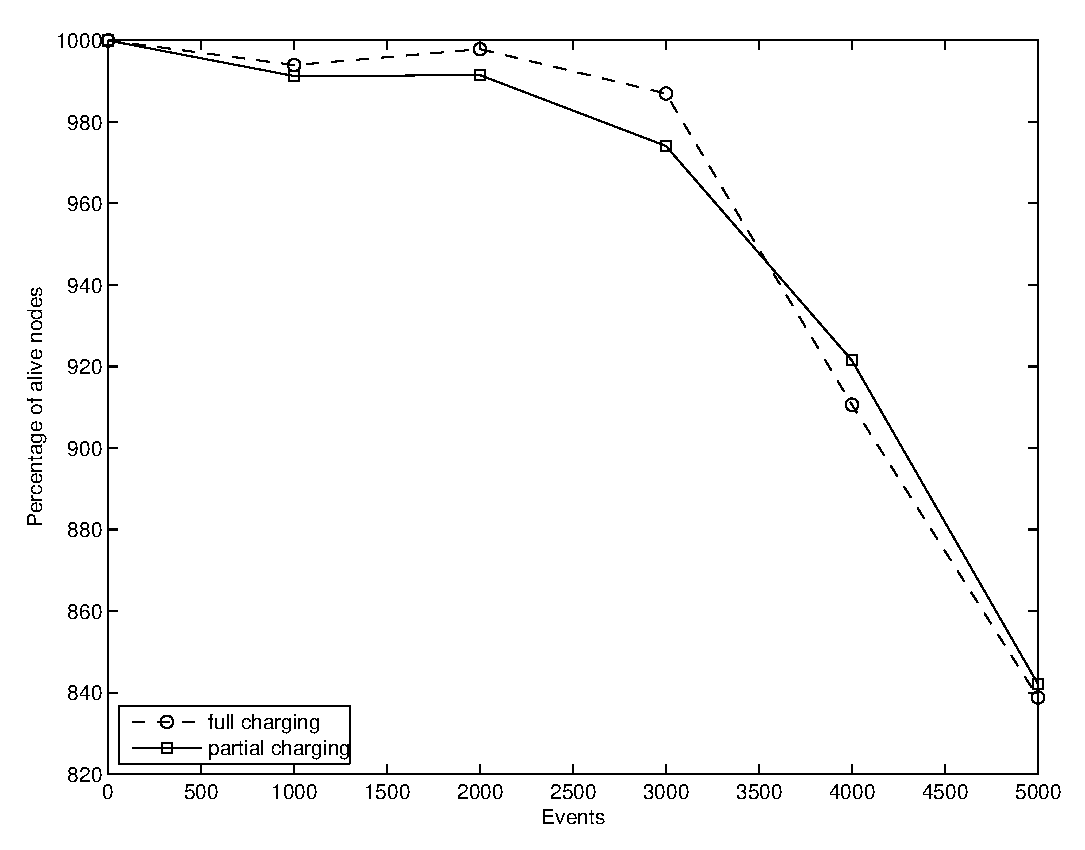
\includegraphics[width=0.32\textwidth]{experiments/classic/2.partialVSfull/alive_nodes_greedy_rc_full-per.eps}}
  \subfloat[Leach]{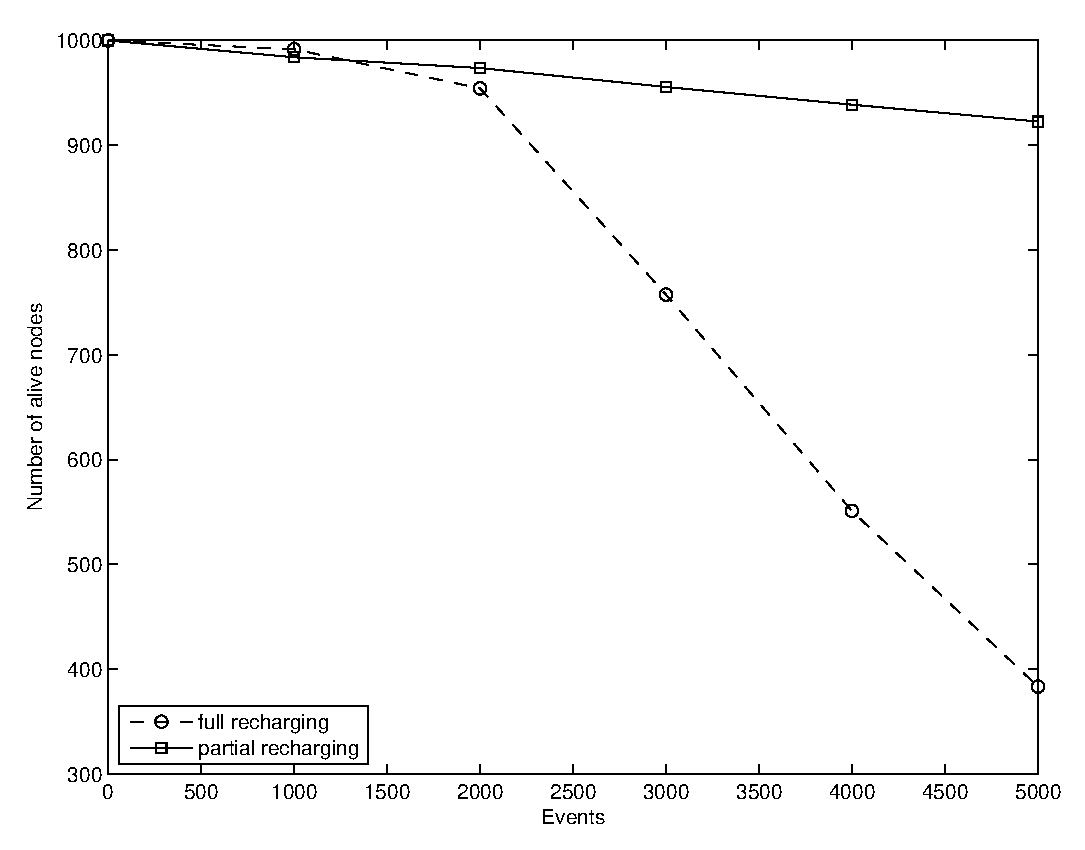
\includegraphics[width=0.32\textwidth]{experiments/classic/2.partialVSfull/alive_nodes_leach_rc_full-per.eps}}
  \subfloat[$\text{E}_{i}$]{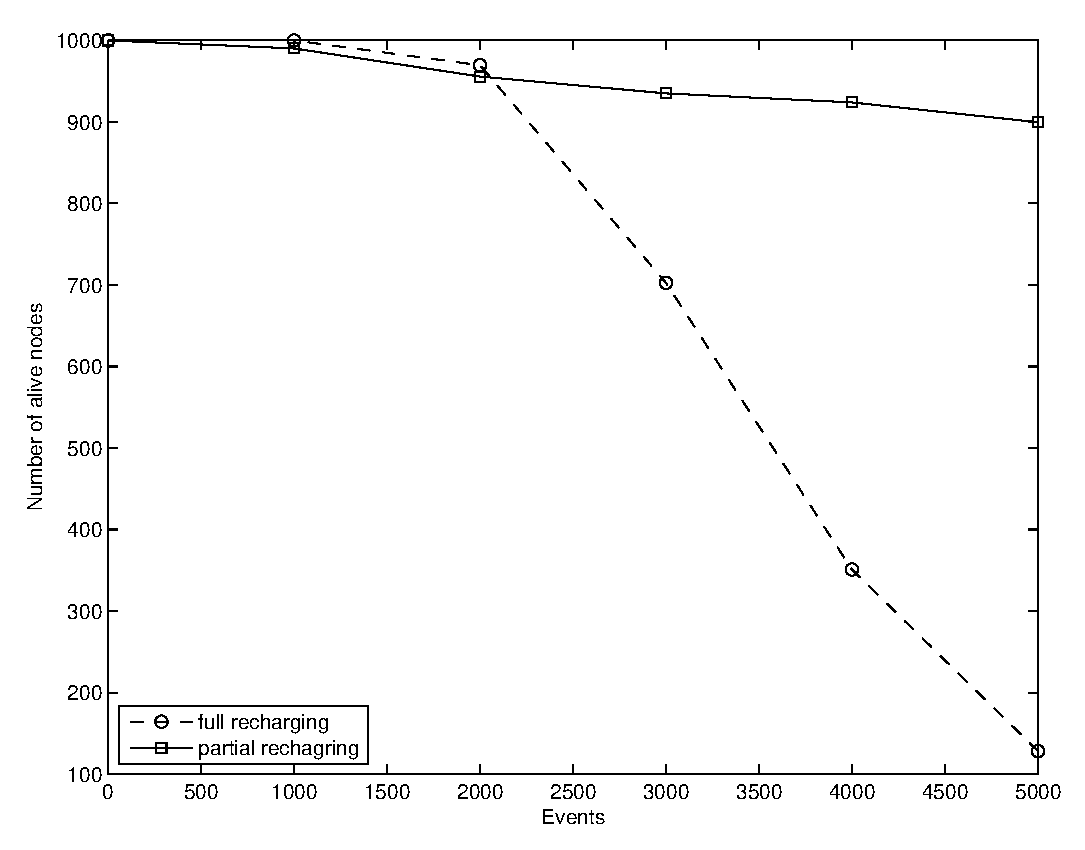
\includegraphics[width=0.32\textwidth]{experiments/classic/2.partialVSfull/alive_nodes_ei_rc_full-per.eps}}
  \caption{Ζωντανοί κόμβοι κατά την πάροδο του χρόνου. Η συνεχόμενη γραμμή αντιστοιχεί στην μερική φόρτιση. Στο Greedy πρωτόκολλο, η πλήρης φόρτιση έχει
ελάχιστα καλύτερα αποτελέσματα. Αυτό συμβαίνει γιατί ο ρυθμός κατανάλωσης των κόμβων που είναι κοντά στην Πηγή είναι πολύ μεγάλος και επομένως συμφέρει να φορτίζονται
πλήρως. Αντίθετα στα άλλα 2 πρωτόκολλα, η μερική φόρτιση
υπερνικάει την στρατηγική της πλήρους φόρτισης.}
  \label{fig:2exp_1_1}
\end{figure}

%%%%%%%%%%%%%%%%%%%%%%%%%%%% 2. CONNECTIVITY %%%%%%%%%%%%%%%%%%%%%%%%%%%%%%%%%%%%%
\begin{figure}[H]
  \centering
  \subfloat[Greedy]{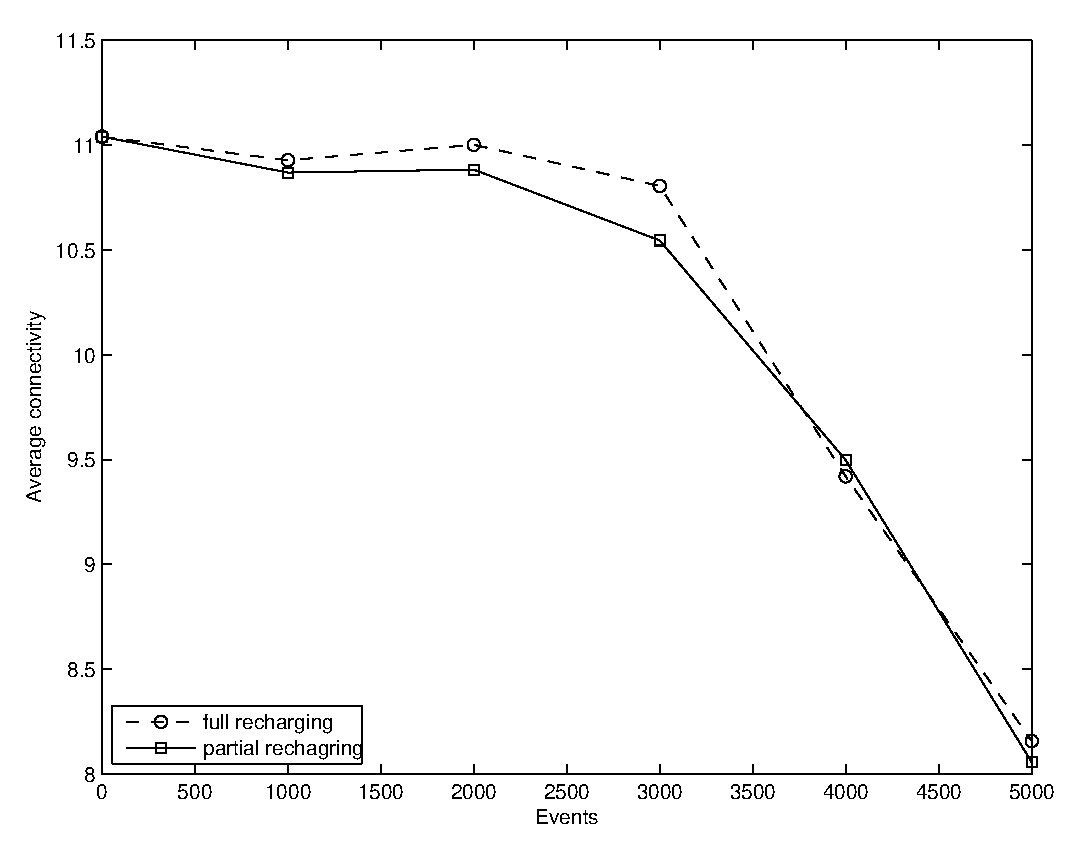
\includegraphics[width=0.32\textwidth]{experiments/classic/2.partialVSfull/connectivity_greedy_rc_full-per.eps}}
  \subfloat[Leach]{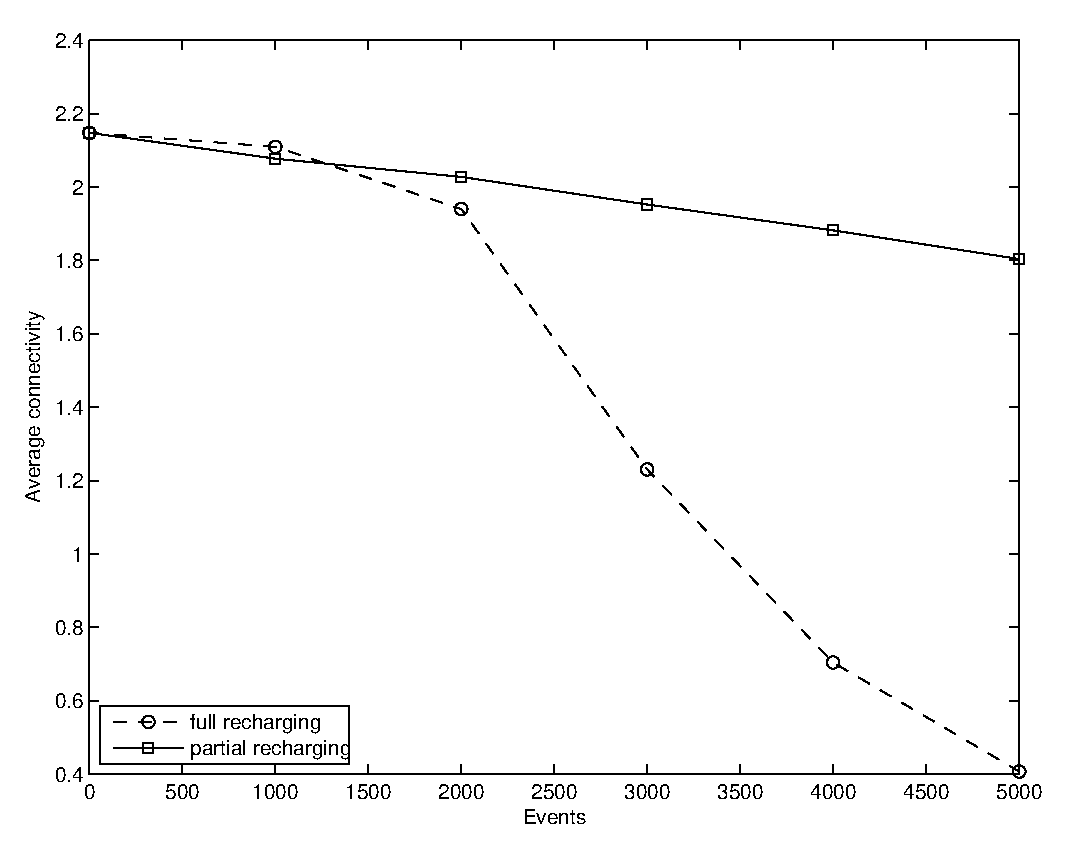
\includegraphics[width=0.32\textwidth]{experiments/classic/2.partialVSfull/connectivity_leach_rc_full-per.eps}}
  \subfloat[$\text{E}_{i}$]{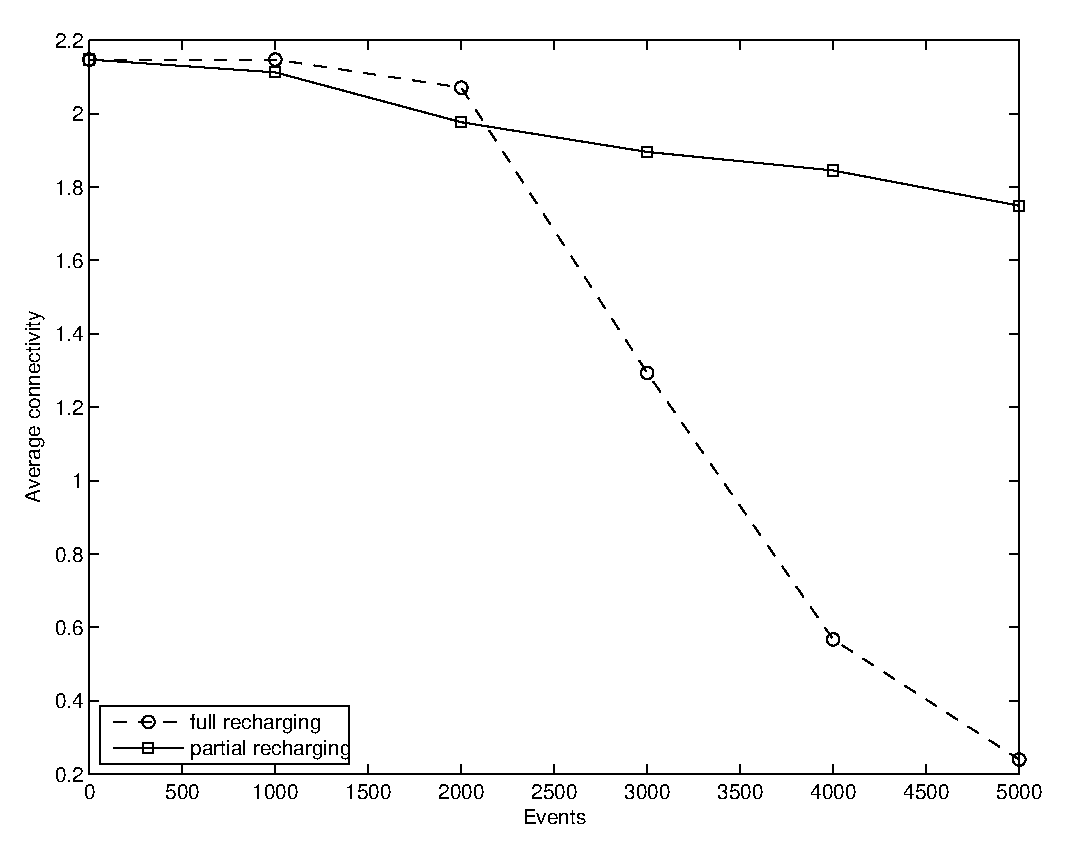
\includegraphics[width=0.32\textwidth]{experiments/classic/2.partialVSfull/connectivity_ei_rc_full-per.eps}}
  \caption{Συνδεσιμότητα κατα την πάροδο του χρόνου. Η συνεχόμενη γραμμή αντιστοιχεί στην μερική φόρτιση. Στο Greedy πρωτόκολλο, η πλήρης φόρτιση έχει ελάχιστα
καλύτερα αποτελέσματα. Αυτό συμβαίνει γιατί ο ρυθμός κατανάλωσης των κόμβων που είναι κοντά στην Πηγή είναι πολύ μεγάλος και επομένως με την μερική φόρτιση οι κόμβοι
πεθαίνουν πιο γρήγορα και το δίκτυο αποσυνδέεται. Αντίθετα στα άλλα 2 πρωτόκολλα, η μερική φόρτιση υπερνικάει την στρατηγική της πλήρους φόρτισης.}
  \label{fig:2exp_2_1}
\end{figure}


%%%%%%%%%%%%%%%%%%%%%%%%%%%% 3. COVERAGE %%%%%%%%%%%%%%%%%%%%%%%%%%%%%%%%%%%%%
\begin{figure}[H]
  \centering
  \subfloat[Greedy με ολική Φόρτιση]{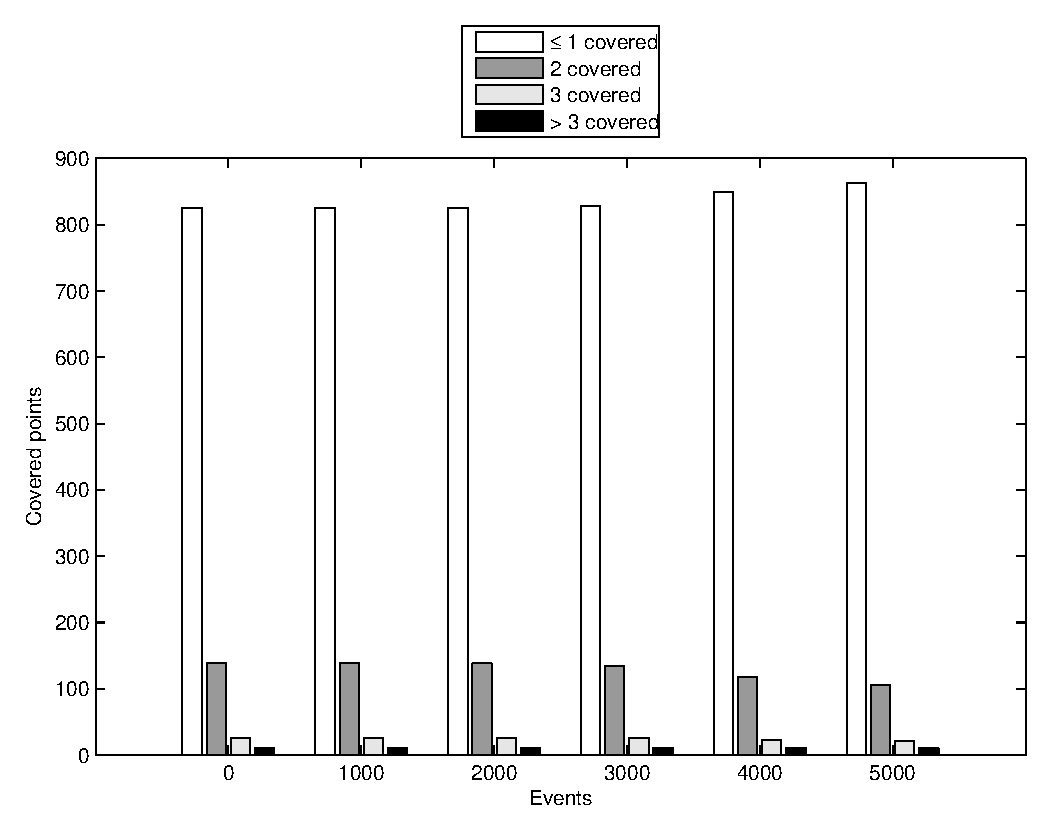
\includegraphics[width=0.48\textwidth]{experiments/classic/2.partialVSfull/coverage_greedy_rc_full.eps}}
  \subfloat[Greedy με μερική Φόρτιση]{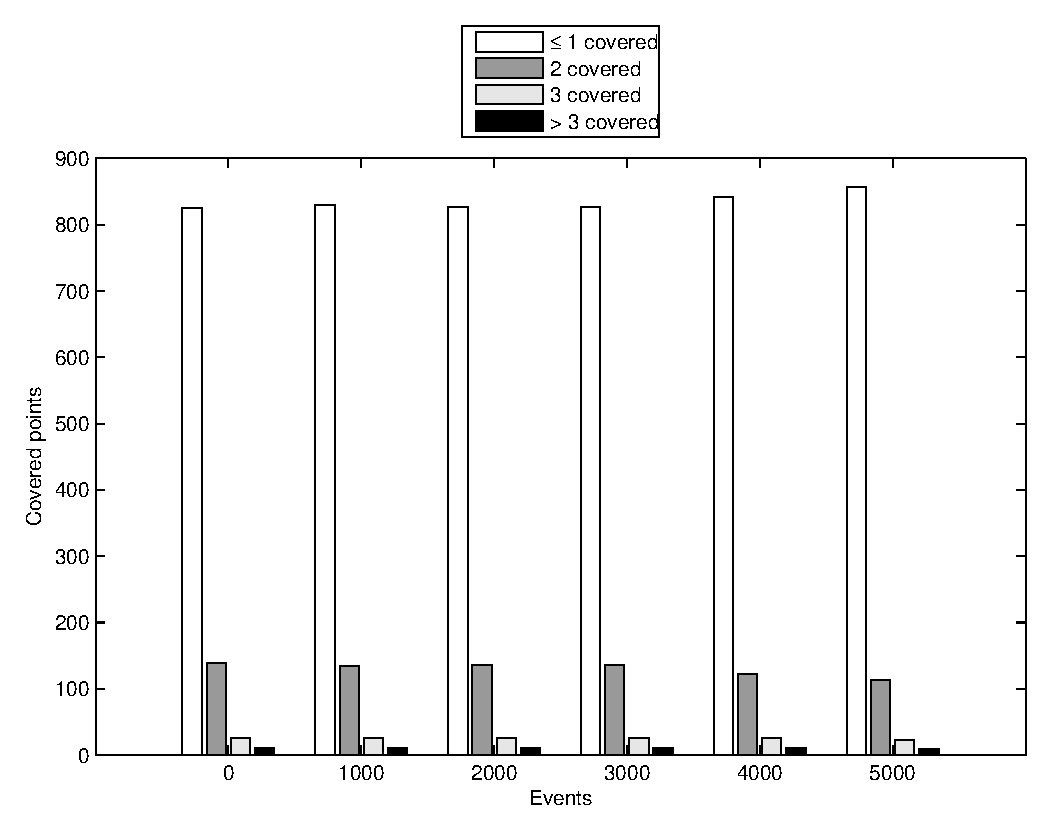
\includegraphics[width=0.48\textwidth]{experiments/classic/2.partialVSfull/coverage_greedy_rc_per.eps}}
  \caption{Κάλυψη του δικτύου κατα την πάροδο του χρόνου για το πρωτόκολλο Greedy. Οι δύο στρατηγικές έχουν παρόμοια αποτελέσματα. Αυτό
συμβαίνει γιατί ο ρυθμός κατανάλωσης των κόμβων που είναι κοντά στην Πηγή είναι πολύ μεγάλος και επομένως η στρατηγική της μερικής φόρτισης δεν αποδίδει καλά.}
  \label{fig:2exp_3_1}
\end{figure}

\begin{figure}[H]
  \centering
  \subfloat[Leach με ολική Φόρτιση]{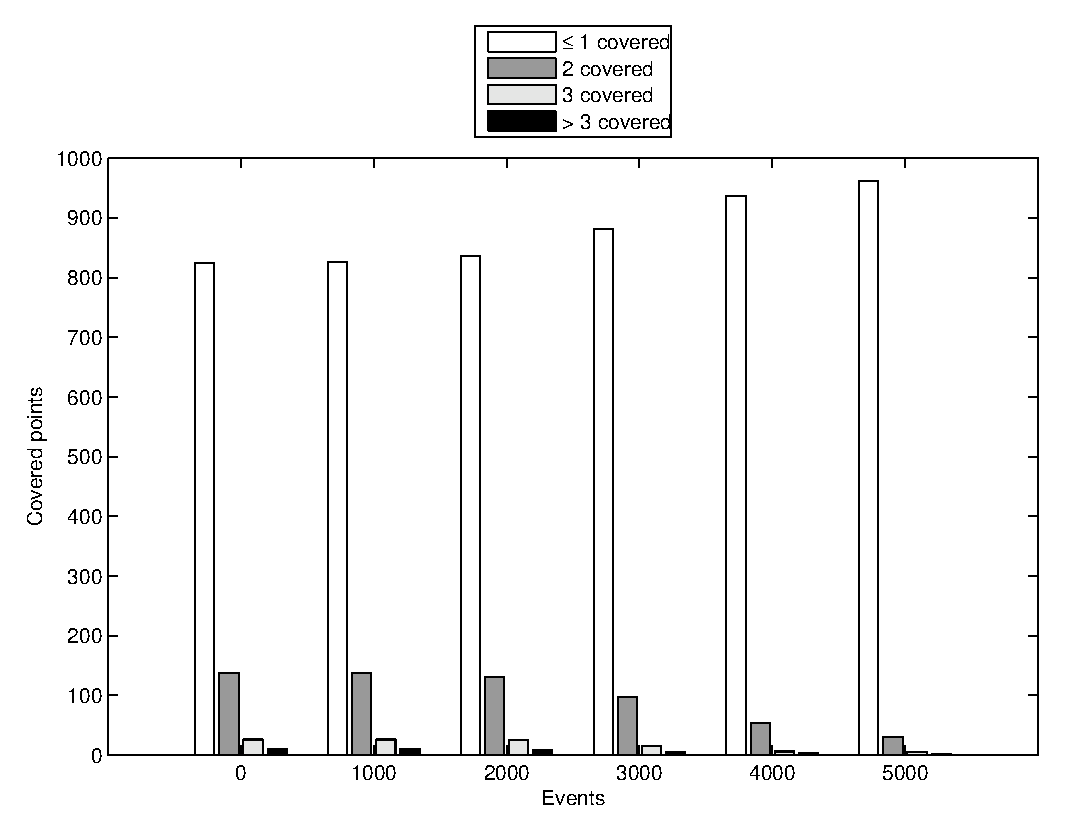
\includegraphics[width=0.48\textwidth]{experiments/classic/2.partialVSfull/coverage_leach_rc_full.eps}}
  \subfloat[Leach με μερική Φόρτιση]{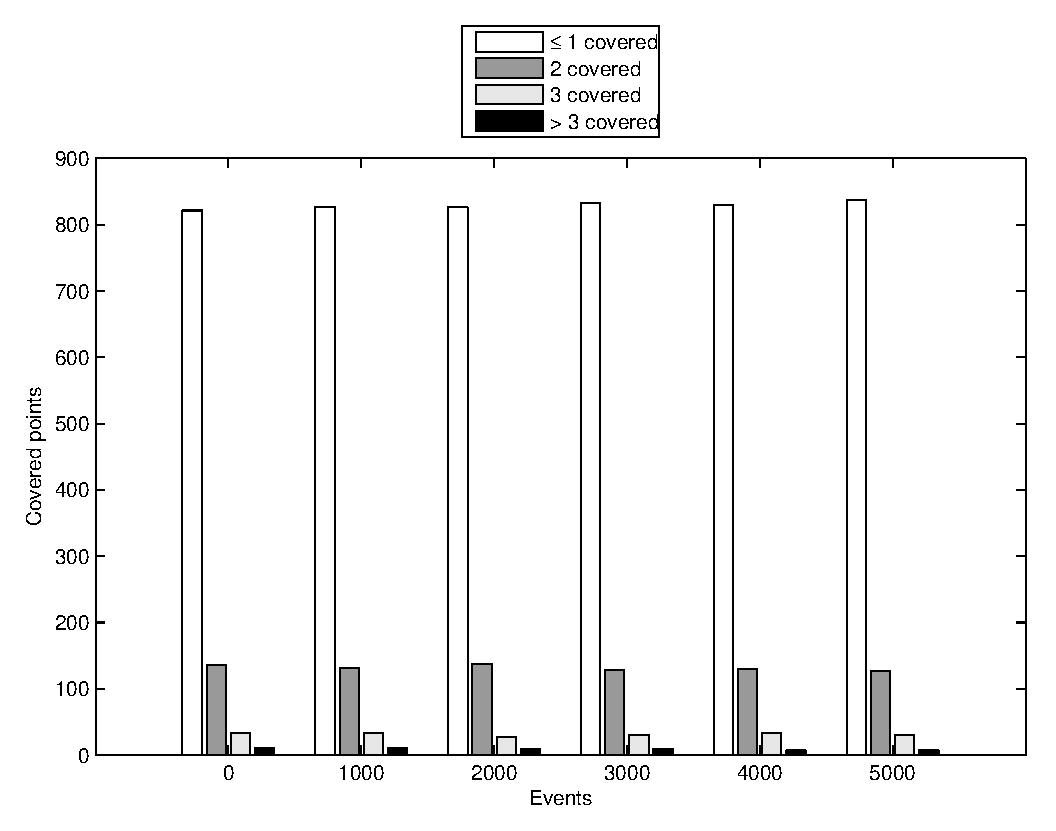
\includegraphics[width=0.48\textwidth]{experiments/classic/2.partialVSfull/coverage_leach_rc_per.eps}}
  \caption{Κάλυψη του δικτύου κατα την πάροδο του χρόνου για το πρωτόκολλο Leach. Είναι εμφανές οτι η στρατηγική της μερικής φόρτισης έχει καλύτερα αποτελέσματα.}
  \label{fig:2exp_3_2}
\end{figure}

\begin{figure}[H]
  \centering
  \subfloat[$\text{E}_{i}$ με ολική Φόρτιση]{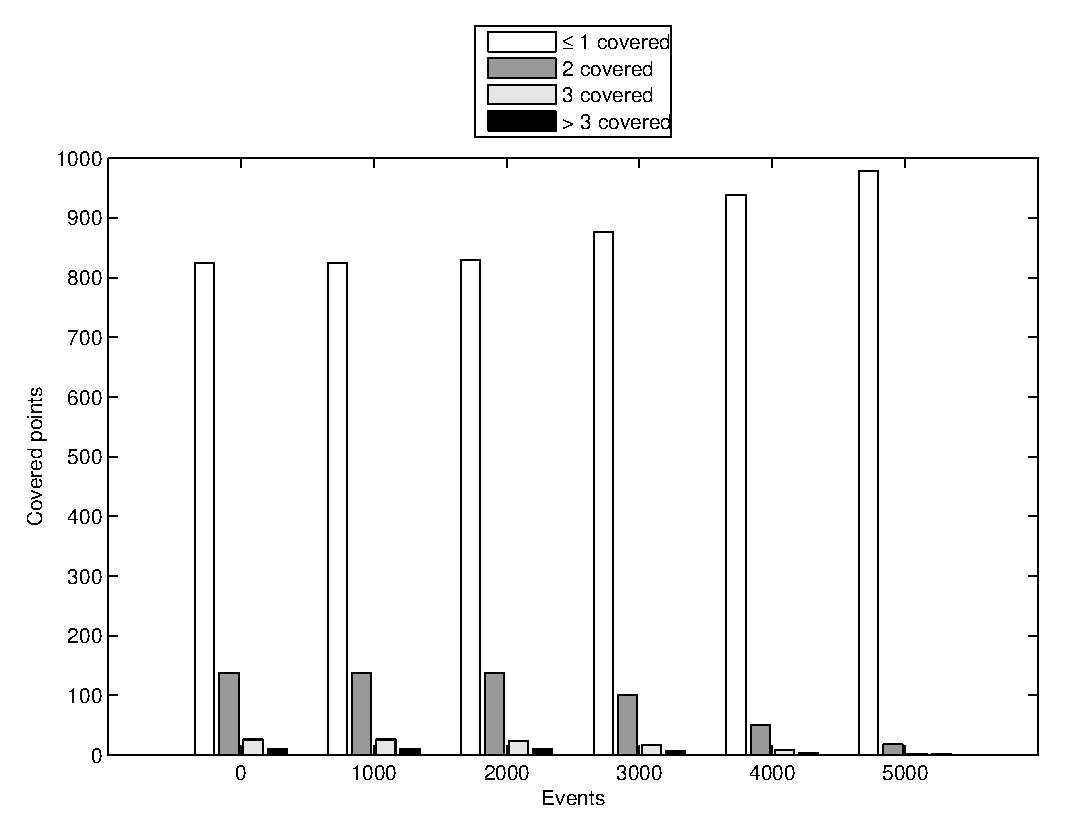
\includegraphics[width=0.48\textwidth]{experiments/classic/2.partialVSfull/coverage_ei_rc_full.eps}}
  \subfloat[$\text{E}_{i}$ με μερική Φόρτιση]{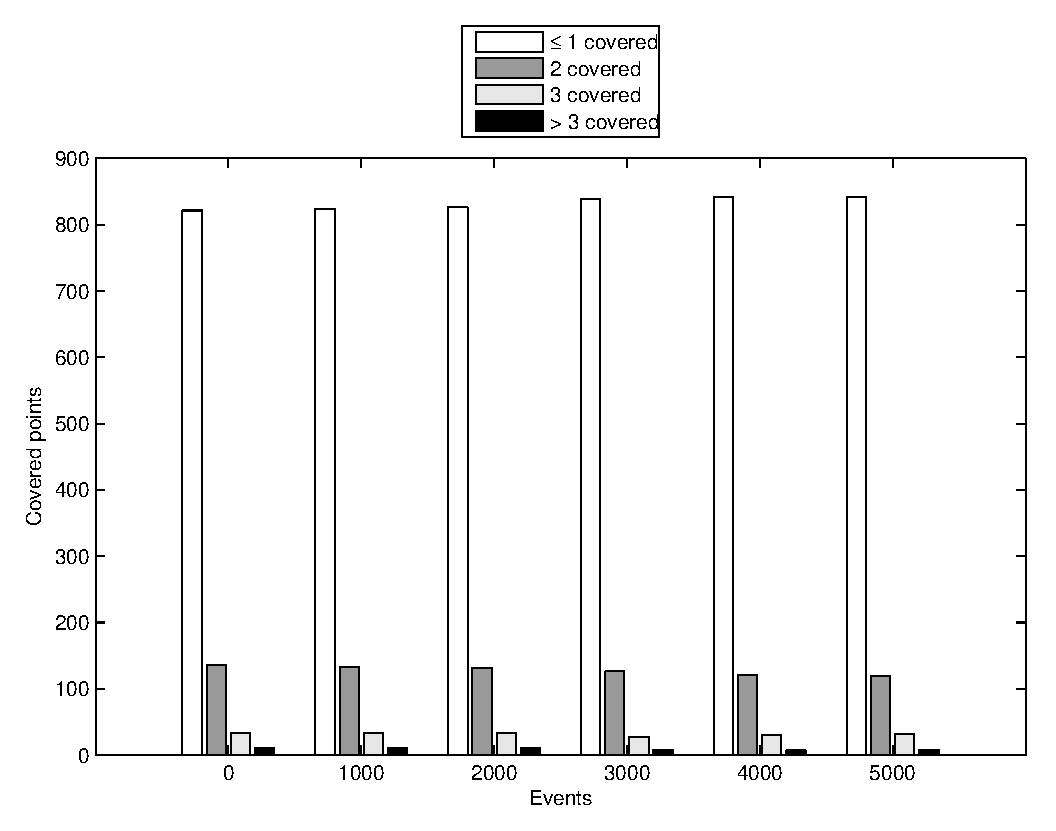
\includegraphics[width=0.48\textwidth]{experiments/classic/2.partialVSfull/coverage_ei_rc_per.eps}}
  \caption{Κάλυψη του δικτύου κατα την πάροδο του χρόνου για το πρωτόκολλο $\text{E}_{i}$. Είναι εμφανές οτι η στρατηγική της μερικής φόρτισης έχει καλύτερα
αποτελέσματα.}
  \label{fig:2exp_3_3}
\end{figure}


\section{Ποσοστό Ενέργειας στον Φορτιστή}\label{sc:result3}
H επόμενη παραμετροποίηση που εξερευνάται είναι η βέλτιστη κατανομή ενέργειας ανάμεσα στον κινητό φορτιστή και τους στατικούς κόμβους σε σχέση με την συνολική αρχική
ενέργεια που διατίθεται στο δίκτυο. Διεξάχθηκαν πειράματα με διάφορες κατανομές ενέργειας και πιο συγκεκριμένα με το 20\%, 40\%, 60\%, και 80\% της συνολικής αρχικής
ενέργειας να δίνεται στον κινητό φορτιστή και το υπόλοιπο στους στατικούς κόμβους. Χρησιμοποιήθηκε ο προσαρμοστικός φορτιστής. Η πειραματική αξιολόγηση έδειξε οτι ένα
ποσοστό κοντά στο 20\% είναι η πιο αποδοτική στρατηγική. Τα αποτελέσματα των πειραμάτων φαίνονται στις εικόνες \ref{fig:3exp_1_1}, \ref{fig:3exp_1_2} και
\ref{fig:3exp_1_3}. Στο Greedy πρωτόκολλο \ref{fig:3exp_1_1}, καθώς ένα μικρό μέρος του δικτύου έχει πολύ μεγάλη κατανάλωση ενέργεια, μια στρατηγική που θα δίνει στον
φορτιστή το 60\% της συνολικής αρχικής ενέργειας του δικτύου φαίνεται να είναι η πιο αποδοτική. Επίσης φαίνεται στην περίπτωση που δοθεί 80\% στον φορτιστή, στην αρχή
πεθαίνουν πολλοί κόμβοι (καθώς έχουν μόνο το 20\% της ενέργειάς τους) αλλά μετά από λίγο ο φορτιστής μπορεί και το επαναφέρει, κυρίως λόγω της φύσης του πρωτοκόλλου
(λίγοι κόμβοι με μεγάλο ρυθμό κατανάλωσης ενέργειας). Αντίθετα στα πρωτόκολλα Leach \ref{fig:3exp_1_2} και $\text{E}_{i}$ \ref{fig:3exp_1_3} μια στρατηγική που δίνει
το 20\%-30\% της αρχικής ενέργειας στον φορτιστή φαίνεται να είναι η βέλτιστη. Επίσης φαίνεται οτι όταν ο φορτιστής έχει το 80\% της ενέργειας επειδή τα πρωτόκολλα
έχουν καλύτερη εξισορρόπηση ενέργειας, ο φορτιστής δεν μπορεί να επαναφέρει το δίκτυο καθώς οι κόμβοι πεθαίνουν πιο κοντά ο ένας στον άλλον από ότι στο Greedy
πρωτόκολλο.



%%%%%%%%%%%%%%%%%%%%%%%%%%%% 1. LIFETIME %%%%%%%%%%%%%%%%%%%%%%%%%%%%%%%%%%%%%
\begin{figure}[H]
  \centering
  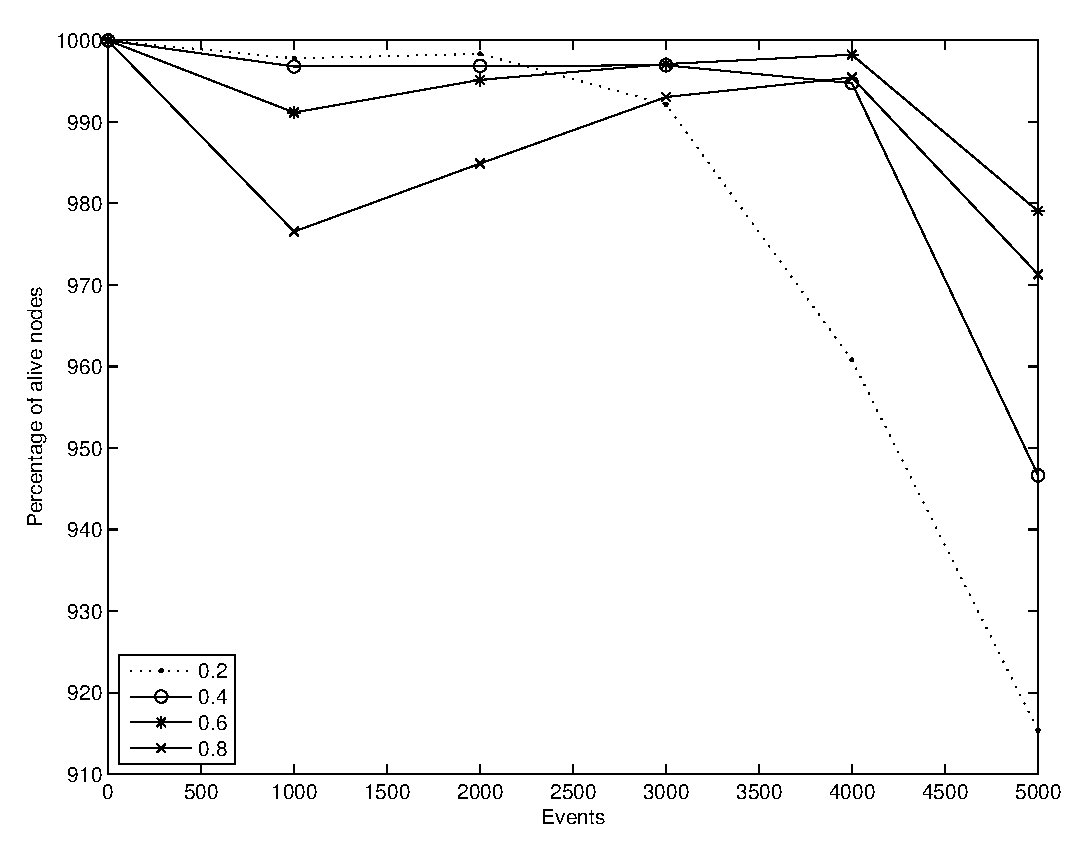
\includegraphics[width=0.9\textwidth]{experiments/classic/3.smallVSbigpercentage/alive_nodes_greedy_rc_per_our.eps}
  \caption{Ζωντανοί κόμβοι κατά την πάροδο του χρόνου στο Greedy πρωτόκολλο με ποικίλα ποσοστά ενέργειας στον κινητό φορτιστή. Μία ποσότητα κοντά στο 60\% στον
φορτιστή φαίνεται να είναι η βέλτιστη, κυρίως λόγω της φύσης του πρωτοκόλλου.}
  \label{fig:3exp_1_1}
\end{figure}

\begin{figure}[H]
  \centering
   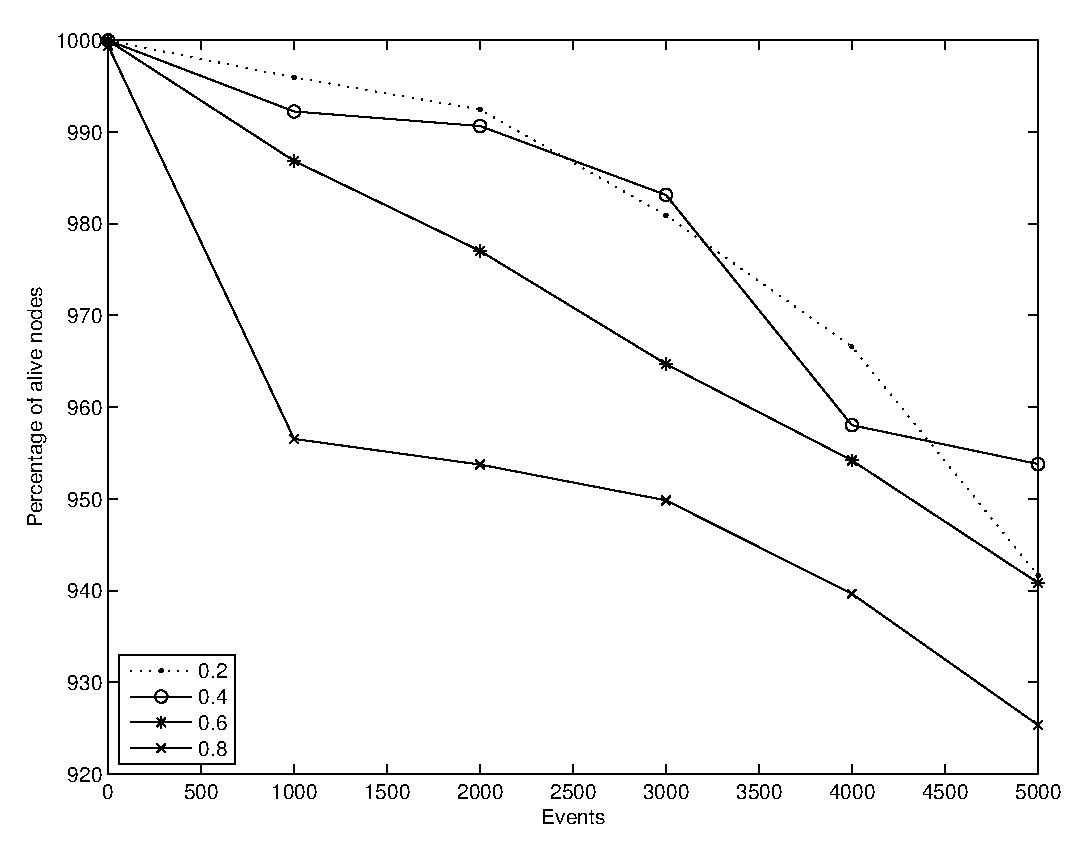
\includegraphics[width=0.9\textwidth]{experiments/classic/3.smallVSbigpercentage/alive_nodes_leach_rc_per_our.eps}
  \caption{Ζωντανοί κόμβοι κατά την πάροδο του χρόνου στο Leach πρωτόκολλο με ποικίλα ποσοστά ενέργειας στον κινητό φορτιστή. Μία ποσότητα κοντά στο 30\% στον
φορτιστή φαίνεται να είναι η βέλτιστη.}
  \label{fig:3exp_1_2}
\end{figure}

\begin{figure}[H]
  \centering
   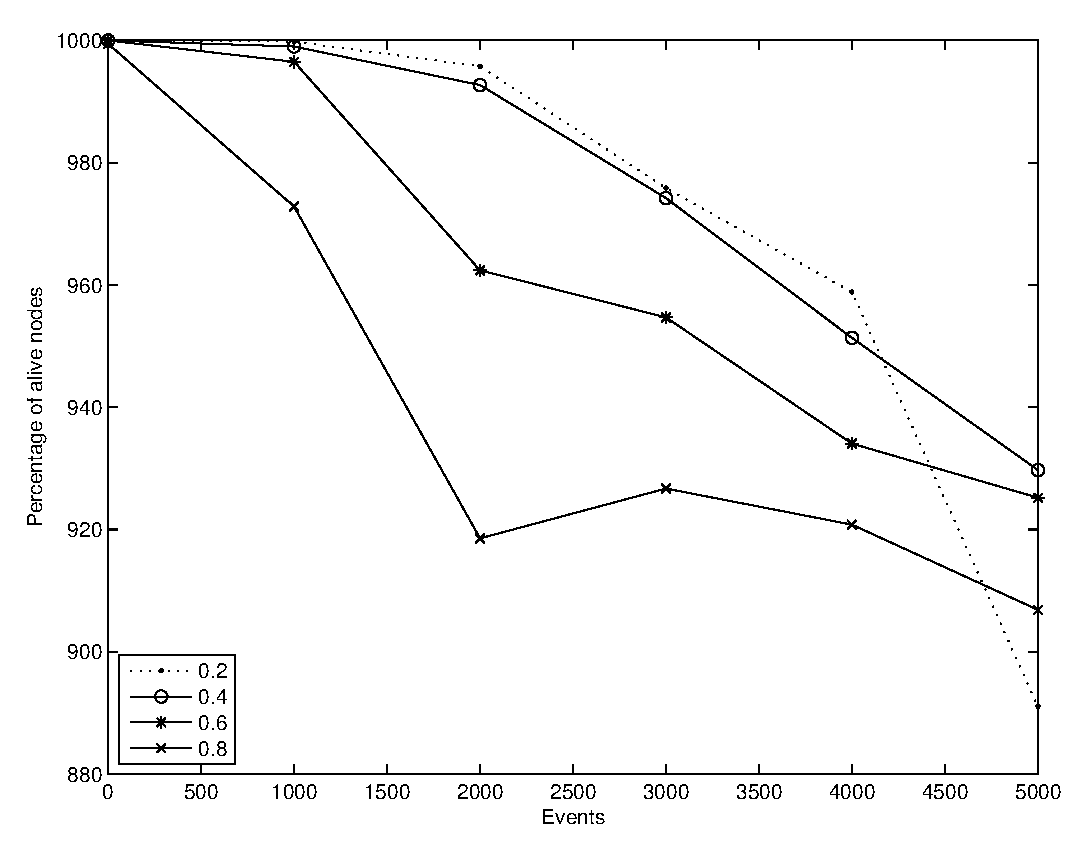
\includegraphics[width=0.9\textwidth]{experiments/classic/3.smallVSbigpercentage/alive_nodes_ei_rc_per_our.eps}
  \caption{Ζωντανοί κόμβοι κατά την πάροδο του χρόνου στο $\text{E}_{i}$ πρωτόκολλο με ποικίλα ποσοστά ενέργειας στον κινητό φορτιστή. Μία ποσότητα κοντά στο 30\%
στον φορτιστή φαίνεται να είναι η βέλτιστη.}
  \label{fig:3exp_1_3}
\end{figure}


\section{Σύγκριση Διαδρομών Φορτιστή}\label{sc:result4}
Αφού έχουν βρεθεί οι βέλτιστες στρατηγικές για τον κινητό φορτιστή (μερική φόρτιση, 20\% της αρχικής ενέργειας), σε αυτήν την ενότητα συγκρίνεται ο προσαρμοστικός
φορτιστής με τον αλγόριθμο καθολικής γνώσης καθώς και με τους υπόλοιπους αφελής αλγορίθμους. Στην πίνακα \ref{tab:dist} φαίνονται οι διαδρομές που καλύπτει ο κάθε
φορτιστής. Όπως φαίνεται ο προσαρμοστικός φορτιστής είναι πολύ κοντά στον φορτιστή καθολικής γνώσεις όσον αφορά την απόσταση που διανύει. Τα αποτελέσματα των
πειραμάτων φαίνονται στις εικόνες \ref{fig:4exp_1_1}, \ref{fig:4exp_1_2}, \ref{fig:4exp_1_3}, \ref{fig:4exp_2_1}, \ref{fig:4exp_2_2} και \ref{fig:4exp_2_3}. Από τα
αποτελέσματα διακρίνεται οτι ο προσαρμοστικός φορτιστής, ενώ χρησιμοποιεί μόνο τοπική πληροφορία, τα πάει αρκετά καλά ειδικά στις περιπτώσεις των πρωτοκόλλων Leach
και $\text{E}_{i}$.

\begin{table}[H]
%\begin{center}
\begin{tabular}{r|c|c|c|}
& Greedy & E$_i$ & LEACH\\\cline{2-4}\cline{2-4}
global knowledge & 48974 & 64330 & 57458\\\cline{2-4}
spiral & 64167 & 64167 & 64167\\\cline{2-4}
random walk & 181135 & 222462 & 222447 \\\cline{2-4}
diameter & 152252 & 172734 & 173169\\\cline{2-4}
adaptive charger & 42412 & 37856 & 38641\\\cline{2-4}
\end{tabular}
%\end{center}
\caption{Distance travelled by chargers}
\label{tab:dist}
\end{table}

%%%%%%%%%%%%%%%%%%%%%%%%%%%% 1. LIFETIME %%%%%%%%%%%%%%%%%%%%%%%%%%%%%%%%%%%%%
\begin{figure}[H]
  \centering
  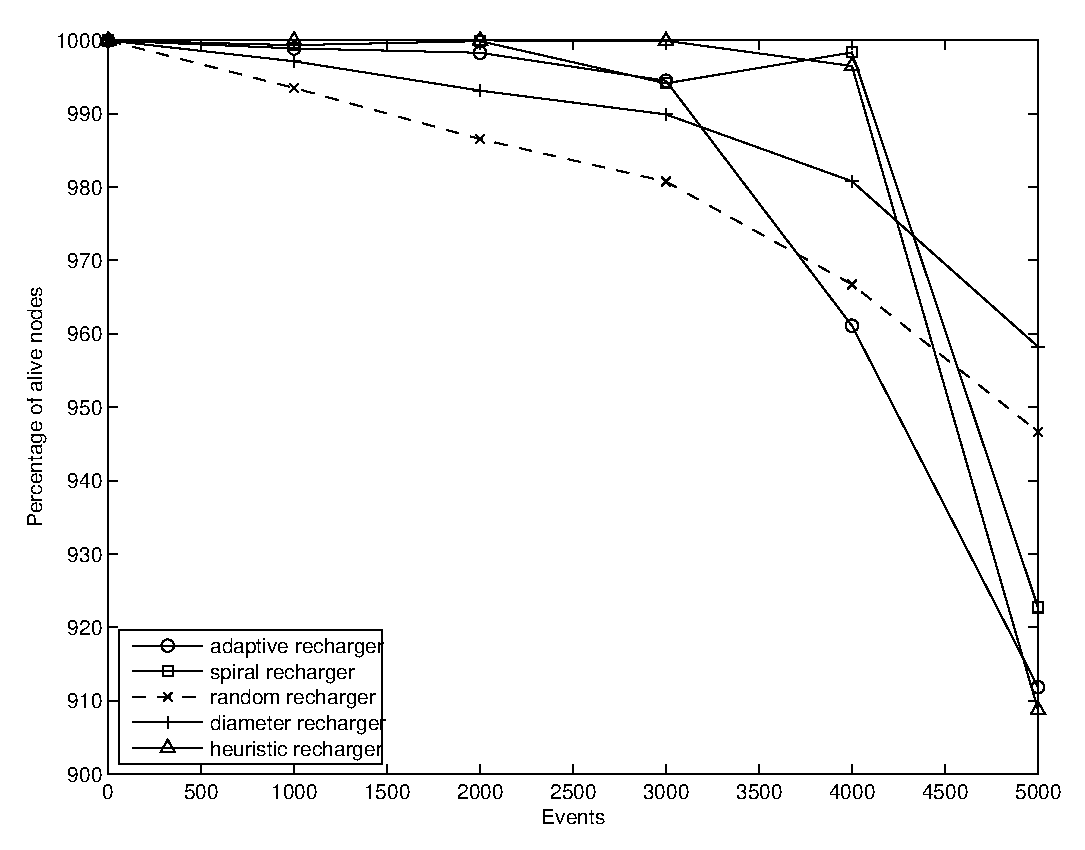
\includegraphics[width=0.9\textwidth]{experiments/classic/4.ourVSnaive/alive_nodes_greedy_rc_per_our-spiral-random-diameter-heuristic.eps}
  \caption{Ζωντανοί κόμβοι κατά την πάροδο του χρόνου στο Greedy πρωτόκολλο για τις διάφορες διαδρομές του κινητού φορτιστή. Χρησιμοποιείται μερική φόρτιση και έχει
δωθεί το 20\% της ενέργειας στον φορτιστή.}
  \label{fig:4exp_1_1}
\end{figure}

\begin{figure}[H]
  \centering
  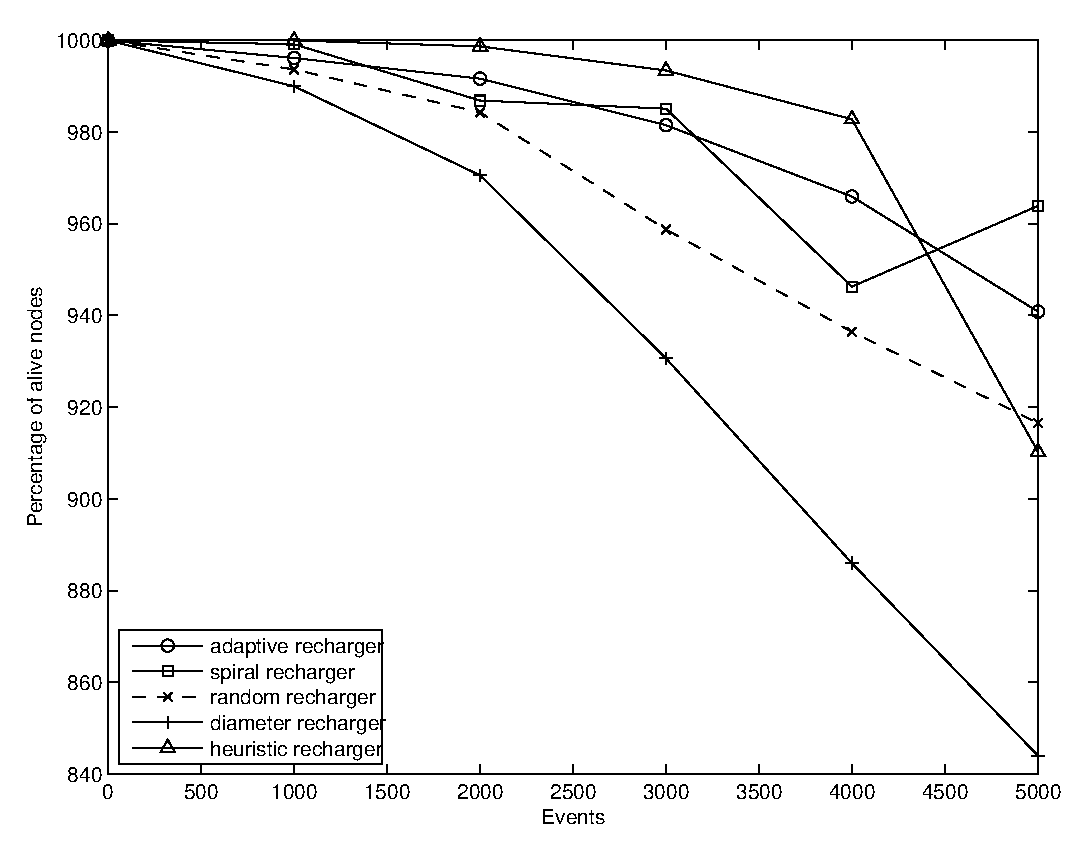
\includegraphics[width=0.9\textwidth]{experiments/classic/4.ourVSnaive/alive_nodes_leach_rc_per_our-spiral-random-diameter-heuristic.eps}
  \caption{Ζωντανοί κόμβοι κατά την πάροδο του χρόνου στο Leach πρωτόκολλο για τις διάφορες διαδρομές του κινητού φορτιστή. Χρησιμοποιείται μερική φόρτιση και έχει
δωθεί το 20\% της ενέργειας στον φορτιστή.}
  \label{fig:4exp_1_2}
\end{figure}

\begin{figure}[H]
  \centering
  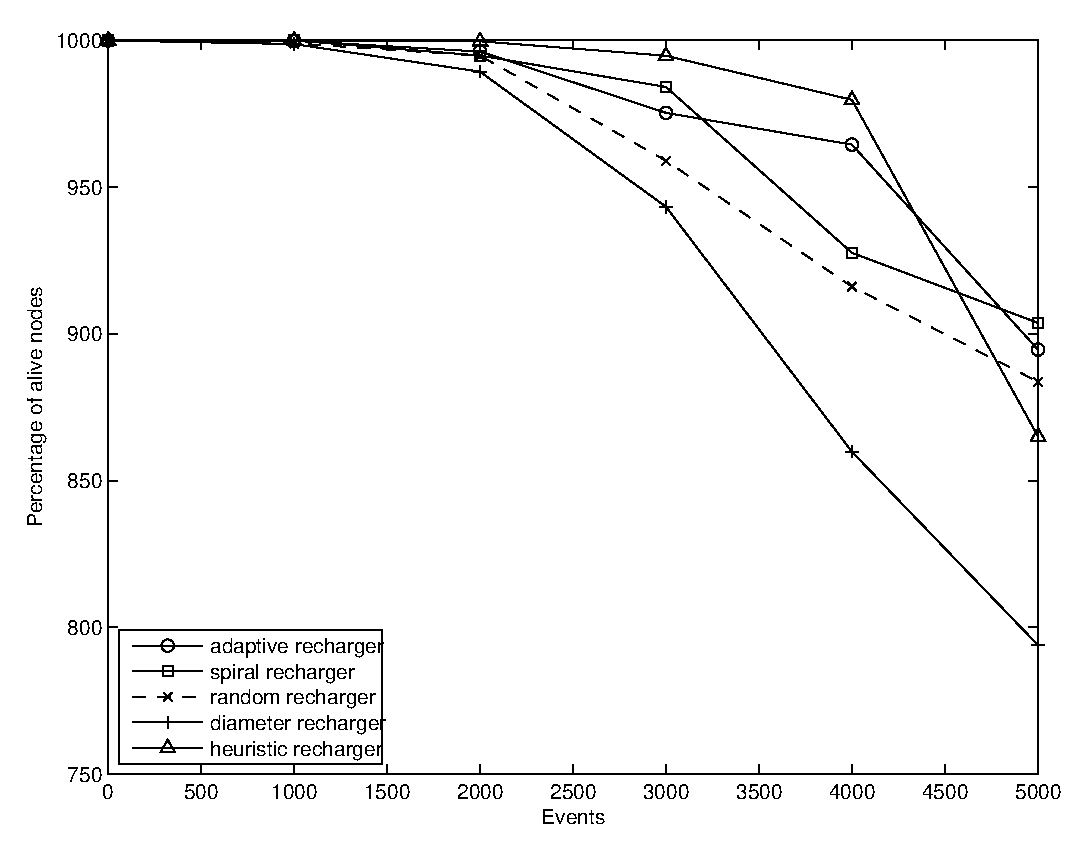
\includegraphics[width=0.9\textwidth]{experiments/classic/4.ourVSnaive/alive_nodes_ei_rc_per_our-spiral-random-diameter-heuristic.eps}
  \caption{Ζωντανοί κόμβοι κατά την πάροδο του χρόνου στο $\text{E}_{i}$ πρωτόκολλο για τις διάφορες διαδρομές του κινητού φορτιστή. Χρησιμοποιείται μερική φόρτιση
και έχει δωθεί το 20\% της ενέργειας στον φορτιστή.}
  \label{fig:4exp_1_3}
\end{figure}



%%%%%%%%%%%%%%%%%%%%%%%%%%%% 2. COVERAGE %%%%%%%%%%%%%%%%%%%%%%%%%%%%%%%%%%%%%
\begin{figure}[H]
  \centering
  \subfloat[Προσαρμοστικός Φορτιστής]{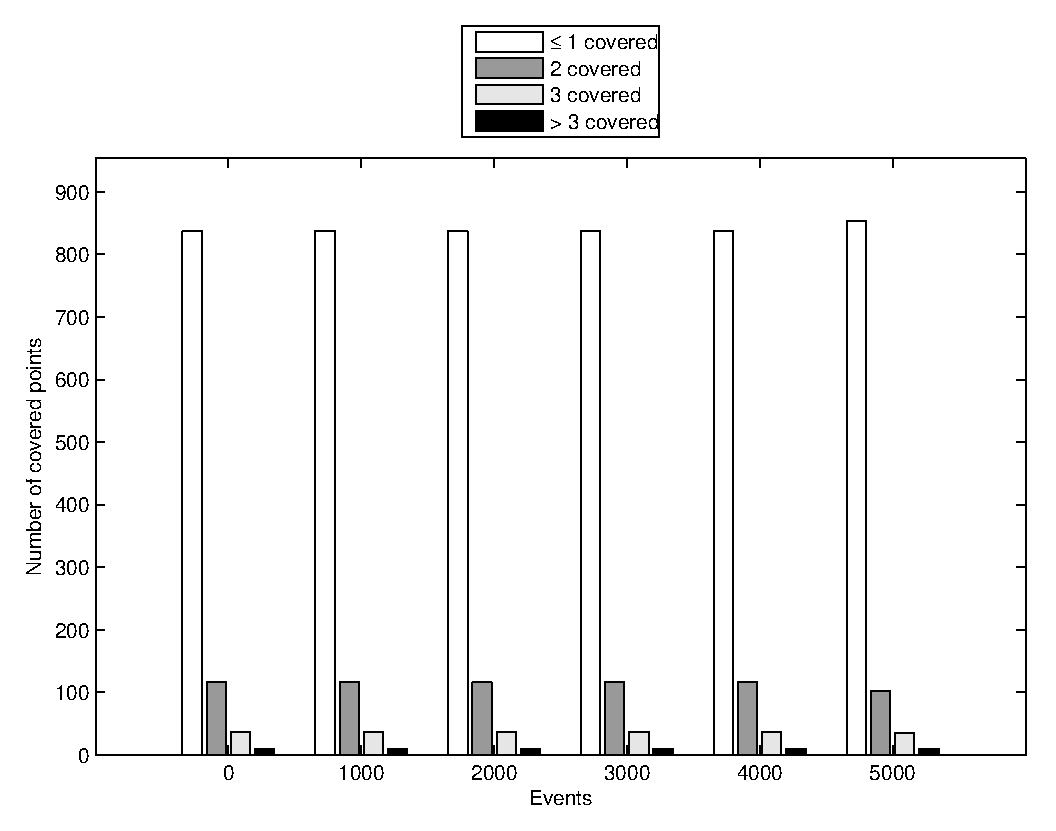
\includegraphics[width=0.48\textwidth]{experiments/classic/4.ourVSnaive/coverage_greedy_rc_per_our.eps}}
  \subfloat[Καθολικής Γνώσης Φορτιστής]{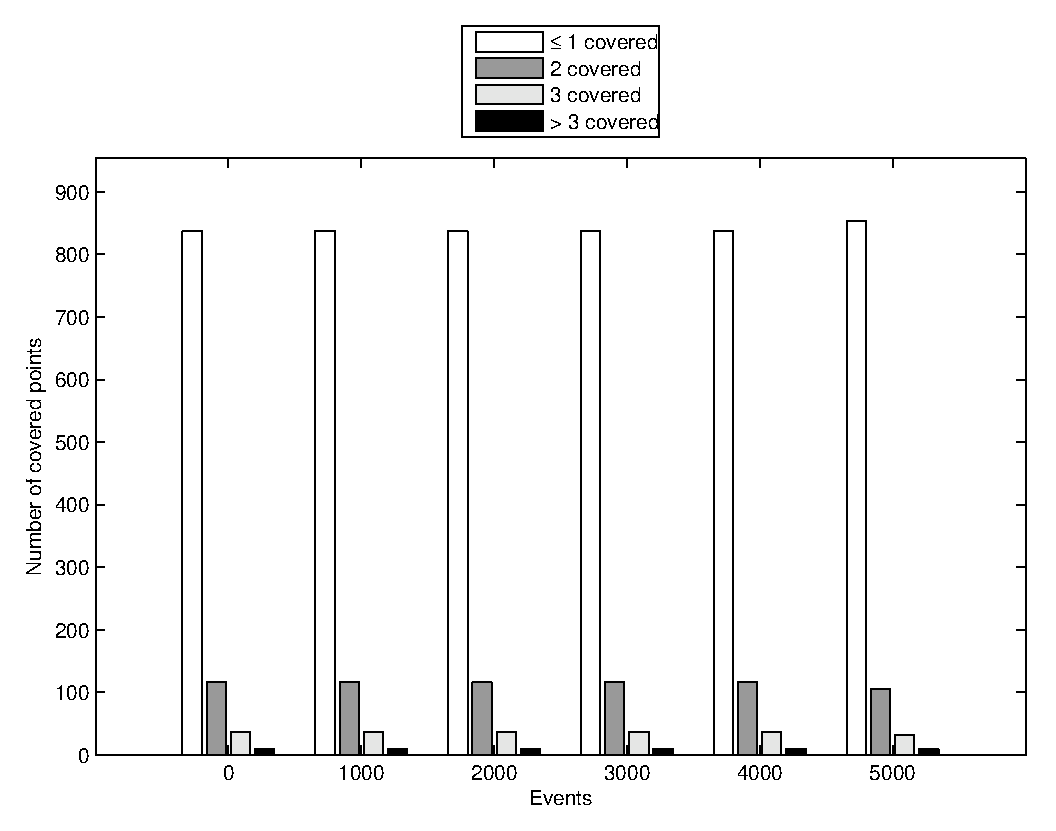
\includegraphics[width=0.48\textwidth]{experiments/classic/4.ourVSnaive/coverage_greedy_rc_per_heuristic.eps}}
  \caption{Κάλυψη του δικτύου κατα την πάροδο του χρόνου για το πρωτόκολλο Greedy. Χρησιμοποιείται μερική φόρτιση και έχει δωθεί το 20\% της ενέργειας στον φορτιστή.}
  \label{fig:4exp_2_1}
\end{figure}

\begin{figure}[H]
  \centering
  \subfloat[Προσαρμοστικός Φορτιστής]{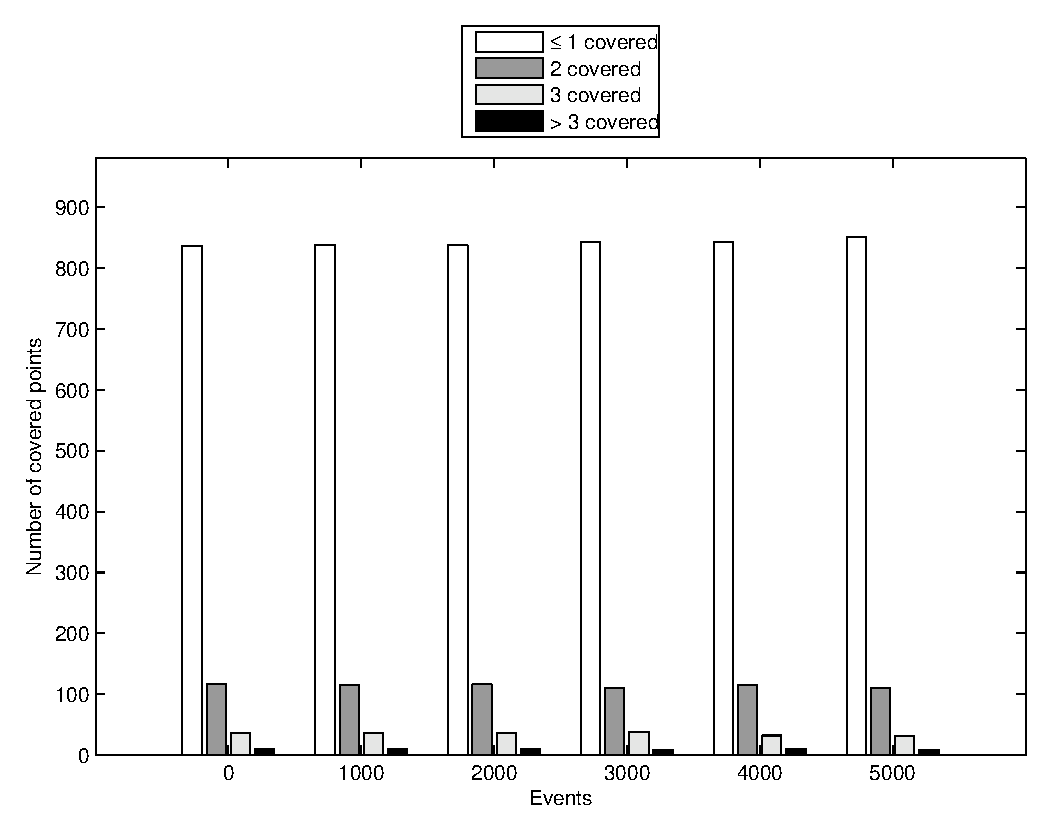
\includegraphics[width=0.48\textwidth]{experiments/classic/4.ourVSnaive/coverage_leach_rc_per_our.eps}}
  \subfloat[Καθολικής Γνώσης Φορτιστής]{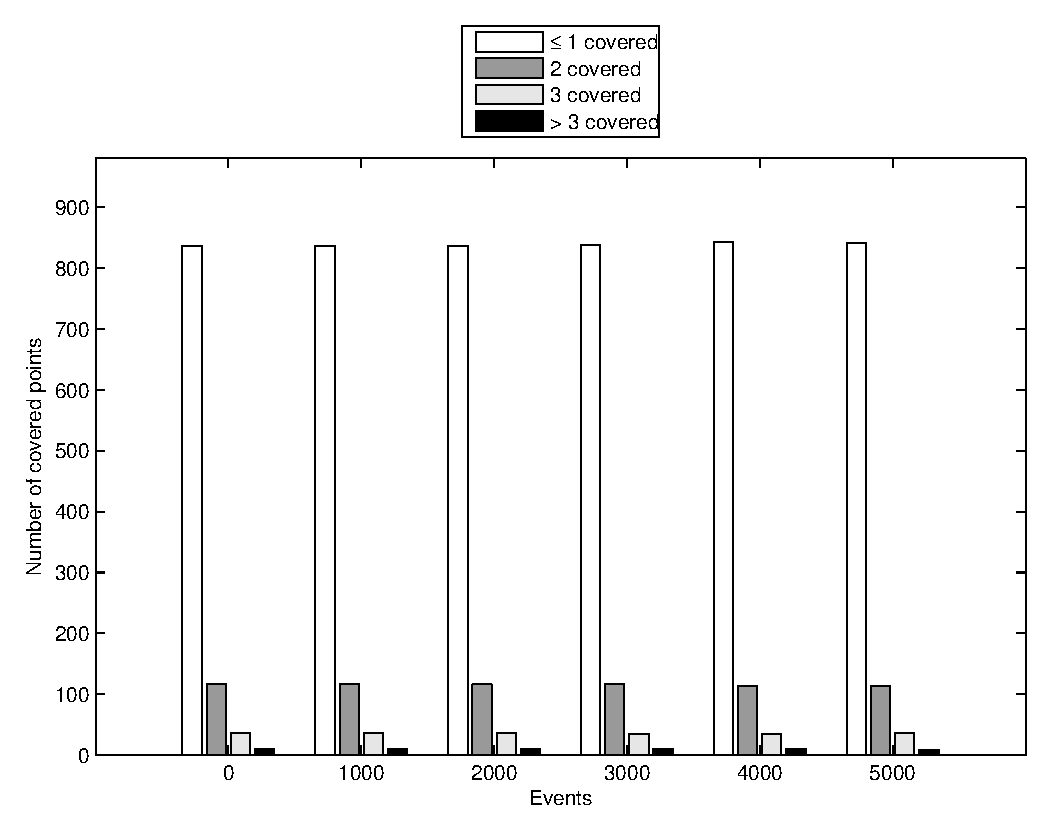
\includegraphics[width=0.48\textwidth]{experiments/classic/4.ourVSnaive/coverage_leach_rc_per_heuristic.eps}}
  \caption{Κάλυψη του δικτύου κατα την πάροδο του χρόνου για το πρωτόκολλο Leach. Χρησιμοποιείται μερική φόρτιση και έχει δωθεί το 20\% της ενέργειας στον φορτιστή.}
  \label{fig:4exp_2_2}
\end{figure}

\begin{figure}[H]
  \centering
  \subfloat[Προσαρμοστικός Φορτιστής]{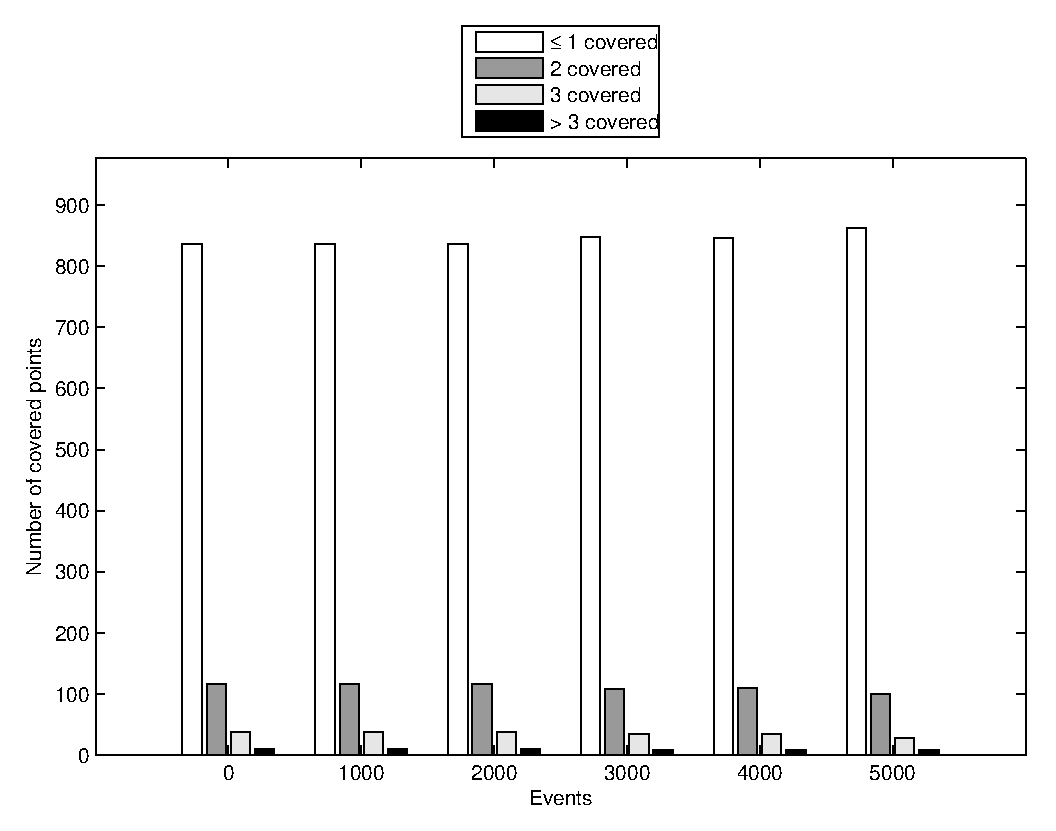
\includegraphics[width=0.48\textwidth]{experiments/classic/4.ourVSnaive/coverage_ei_rc_per_our.eps}}
  \subfloat[Καθολικής Γνώσης Φορτιστής]{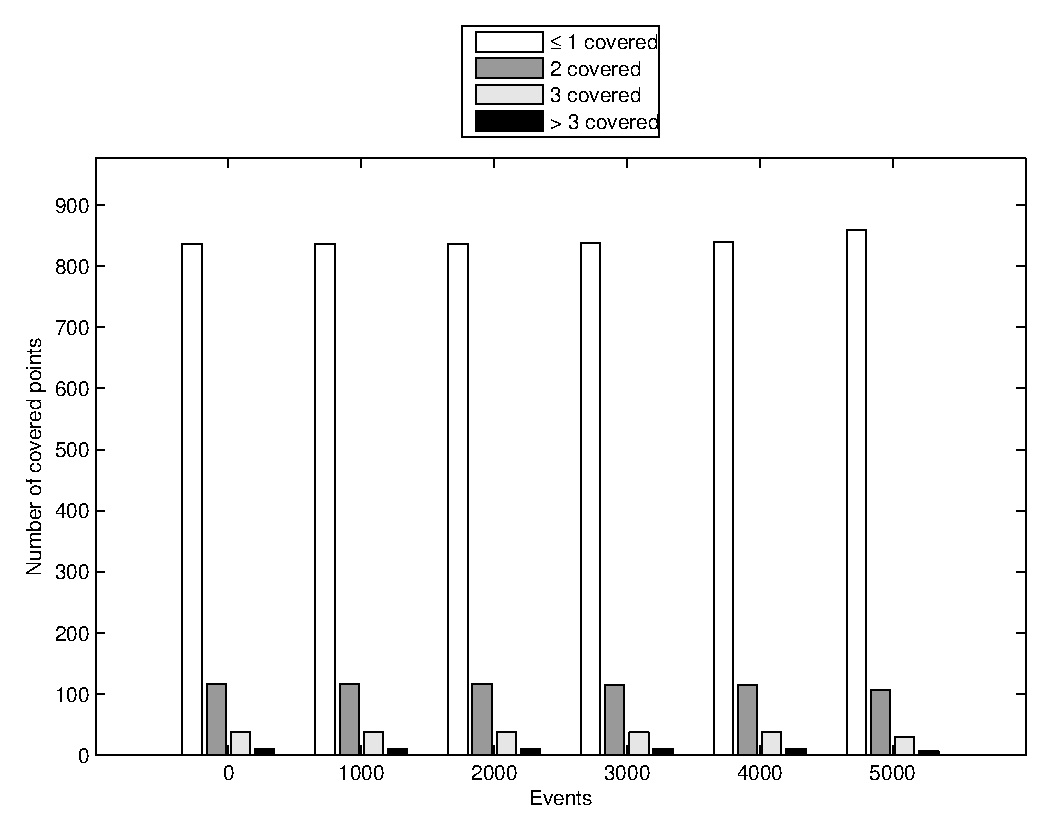
\includegraphics[width=0.48\textwidth]{experiments/classic/4.ourVSnaive/coverage_ei_rc_per_heuristic.eps}}
  \caption{Κάλυψη του δικτύου κατα την πάροδο του χρόνου για το πρωτόκολλο $\text{E}_{i}$. Χρησιμοποιείται μερική φόρτιση και έχει
δωθεί το 20\% της ενέργειας στον φορτιστή.}
  \label{fig:4exp_2_3}
\end{figure}























\section{Αυξάνοντας τον αριθμό των κόμβων}\label{sc:result5}
Σε αυτό το πείραμα, ο αριθμός των κόμβων αυξάνεται δραματικά. Συγκεκριμένα από 1000 κόμβους που ήταν στα προηγούμενα πειράματα, ο αριθμός των κόμβων γίνεται 4000. Ο
κινητός φορτιστής πλέον τώρα έχει να εξυπηρετήσει 4 φορές παραπάνω κόμβους. Το πείραμα αυτό προσπαθεί να διαπιστώσει αν η αρχιτεκτονική του δικτύου που σχεδιάστηκε
στις προηγούμενες ενότητες έχει κάποια όρια στην εξυπηρέτηση των κόμβων. Τα αποτελέσματα δείχνουν οτι γενικώς ο φορτιστής μπορεί να βελτιώσει τις μετρικές του
δικτύου αλλά σε περιορισμένο βαθμό και φυσικά με μικρότερη απόδοση σε σχέση με τα προηγούμενα πειράματα και τους 1000 κόμβους. Από τα αποτελέσματα των πειραμάτων
στην εικόνα \ref{fig:5_1exp_1_1}, ο κινητός φορτιστής επεκτείνει τον χρόνο ζωής του δικτύου αλλά εμφανίζεται μια μικρή
αστάθεια ως προς το πλήθος των ζωντανών κόμβων κατα την διάρκεια του χρόνου ζωής του δικτύου. Αυτό προιδεάζει οτι η απόδοση του κινητού φορτιστή θα είναι χειρότερη
σε αυτή την σειρά των πειραμάτων σε σχέση με τις προηγούμενες λόγω του αυξημένου αριθμού των κόμβων και δημιουγεί νέα κατεύθυνση έρευνας που θα διαχειρίζεται
πολλαπλούς κινητούς κόμβους για καλύτερη διαχείρηση της συνολικής ενέργειας του δικτύου.

\subsection{Με και Χωρίς Φόρτιση}\label{subc:result5_1}
%%%%%%%%%%%%%%%%%%%%%%%%%%%% 1. LIFETIME %%%%%%%%%%%%%%%%%%%%%%%%%%%%%%%%%%%%%
\begin{figure}[H]
  \centering
  \subfloat[Greedy]{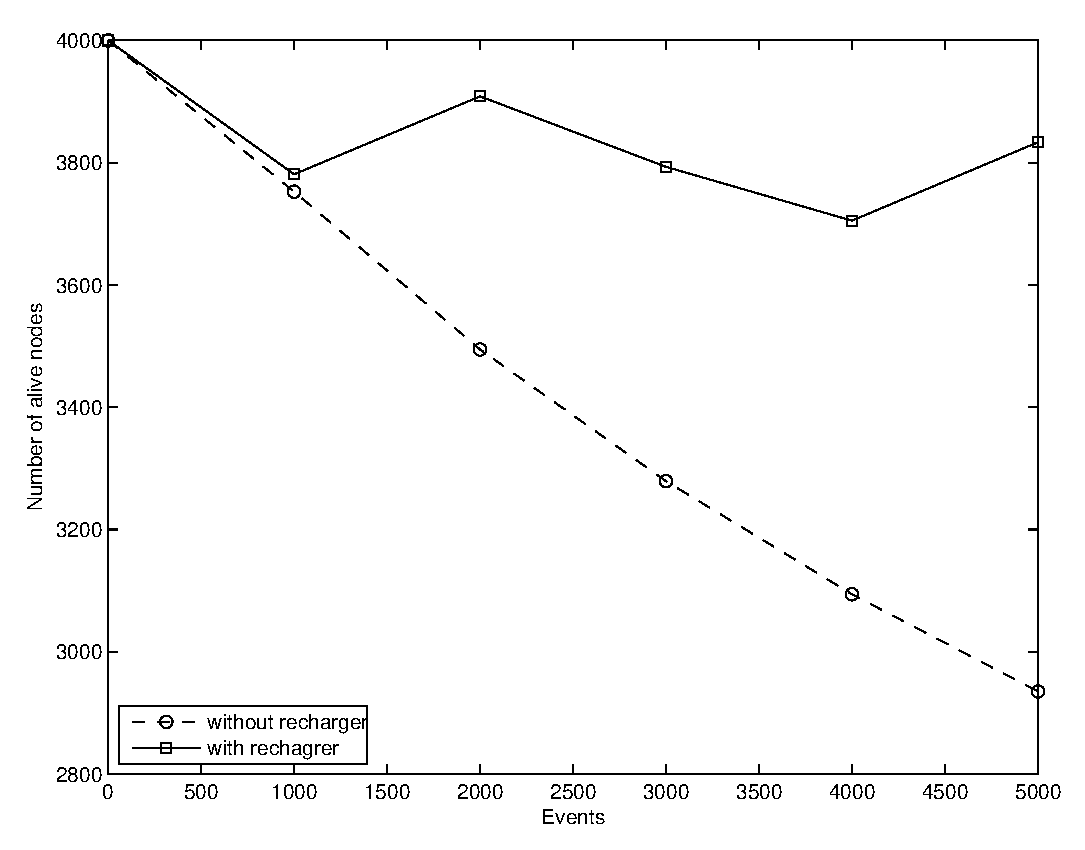
\includegraphics[width=0.32\textwidth]{experiments/4000nodes/1.norechargeVSrecharge/alive_nodes_greedy_nonrc-rc.eps}}
  \subfloat[Leach]{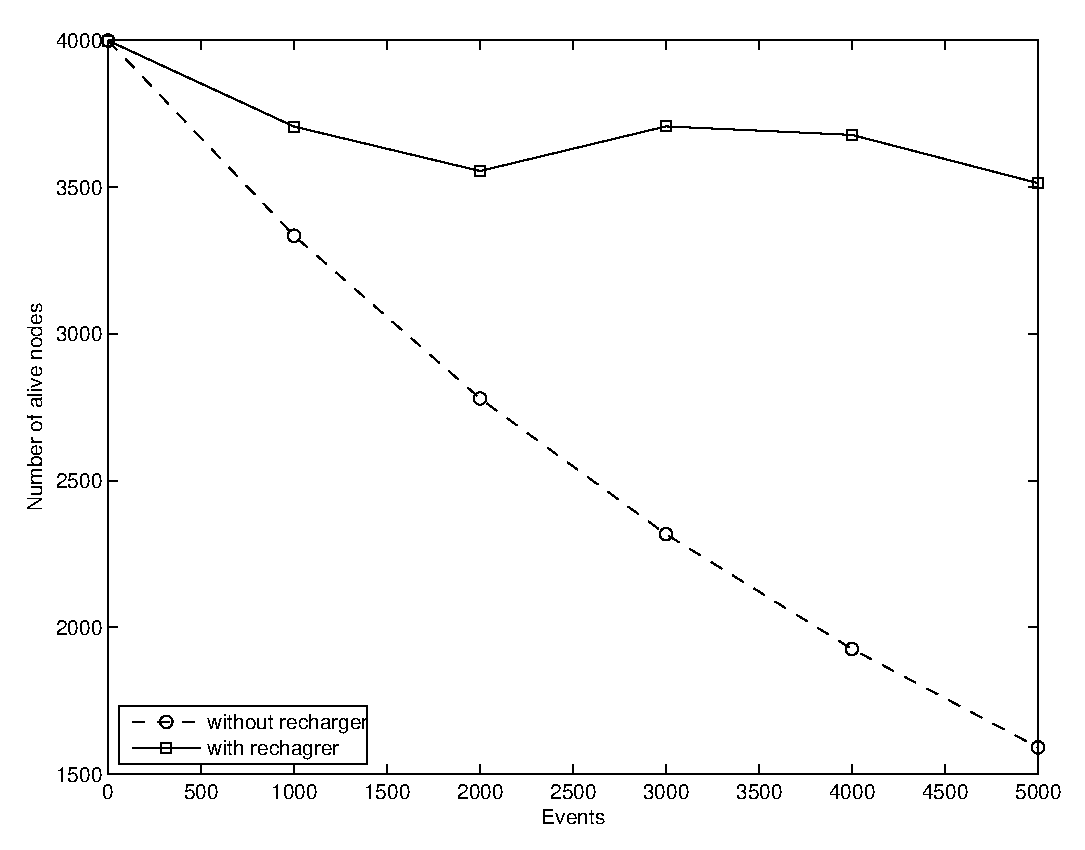
\includegraphics[width=0.32\textwidth]{experiments/4000nodes/1.norechargeVSrecharge/alive_nodes_leach_nonrc-rc.eps}}
  \subfloat[$E_{i}$]{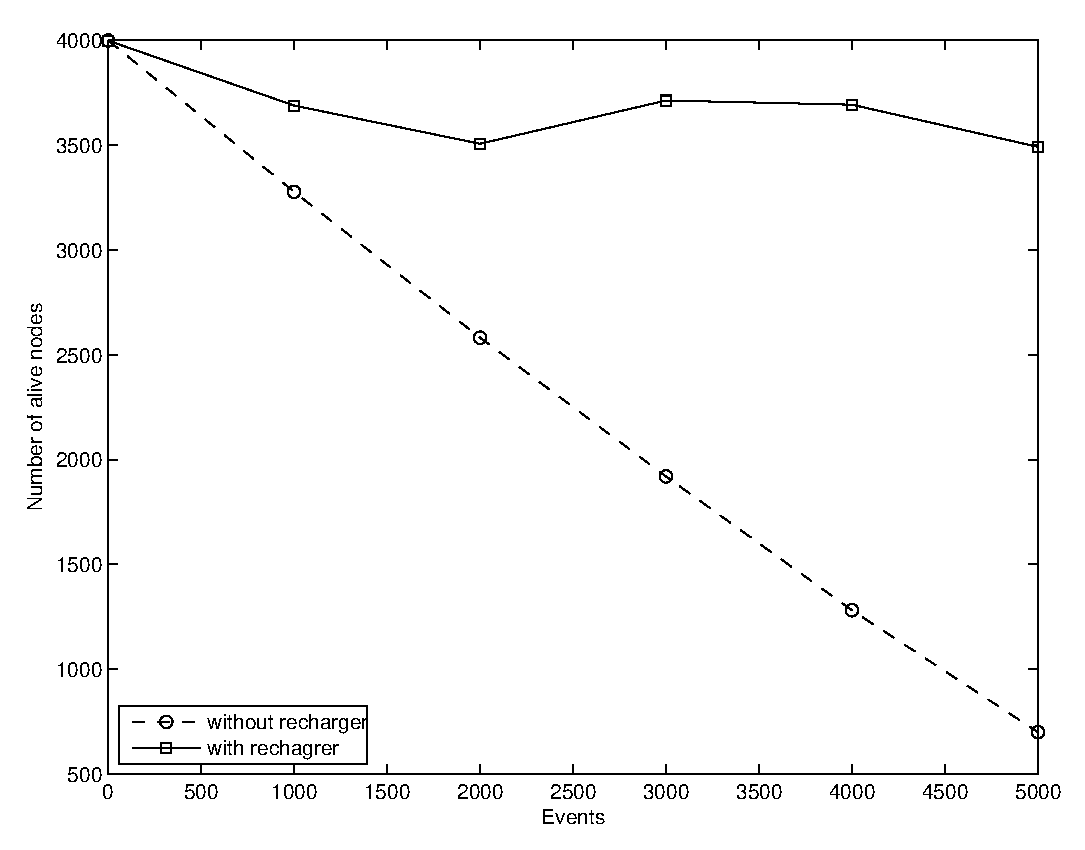
\includegraphics[width=0.32\textwidth]{experiments/4000nodes/1.norechargeVSrecharge/alive_nodes_ei_nonrc-rc.eps}}
  \caption{Ζωντανοί κόμβοι κατά την πάροδο του χρόνου. Η συνεχόμενη γραμμή αντιστοιχεί στο δίκτυο με κινητό φορτιστή. Γίνεται εμφανές οτι γενικά υπάρχει αύξηση
	του χρόνου ζωής του δικτύου αν δοθεί μέρος της συνολικής ενέργειας στον φορτιστή αλλά δεν υπάρχει τόση καλή ισορροπία όπως στις μετρήσεις της ενότητας
\ref{sc:result1}.}
  \label{fig:5_1exp_1_1}
\end{figure}


%%%%%%%%%%%%%%%%%%%%%%%%%%%% 3. COVERAGE %%%%%%%%%%%%%%%%%%%%%%%%%%%%%%%%%%%%%

\begin{figure}[H]
  \centering
  \subfloat[Greedy]{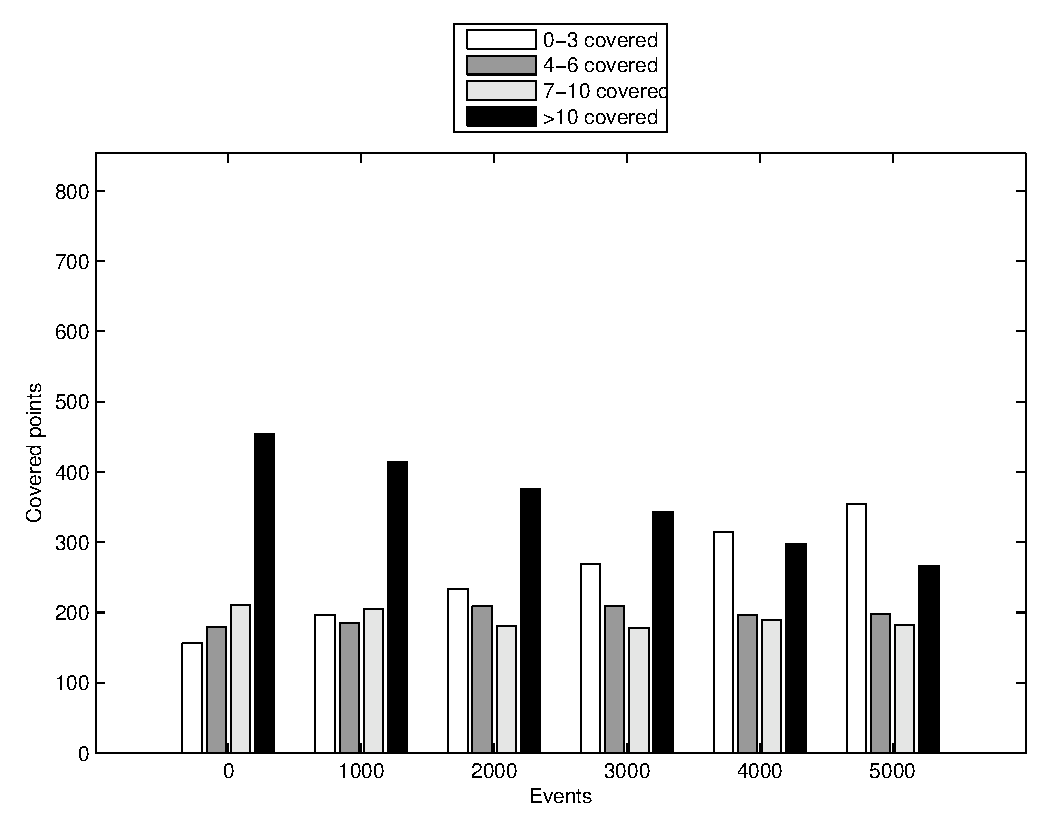
\includegraphics[width=0.48\textwidth]{experiments/4000nodes/1.norechargeVSrecharge/coverage_greedy.eps}}
  \subfloat[Greedy με Φορτιστή]{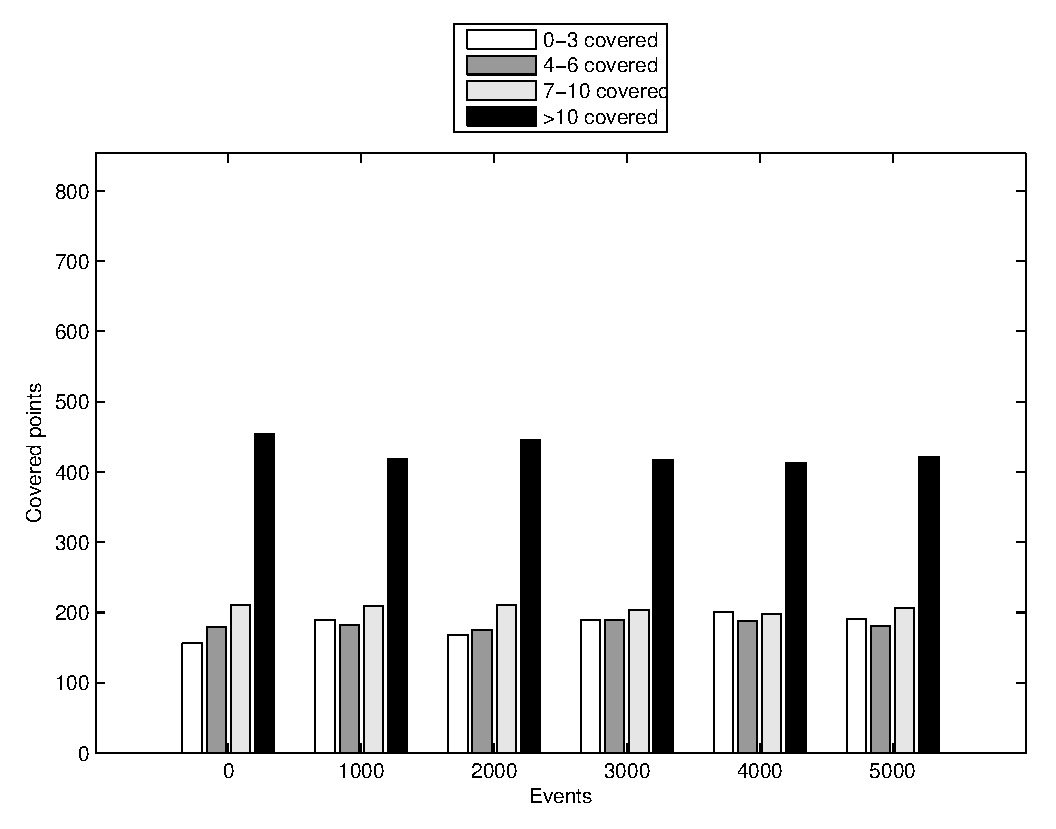
\includegraphics[width=0.48\textwidth]{experiments/4000nodes/1.norechargeVSrecharge/coverage_greedy_rc.eps}}
  \caption{Κάλυψη του δικτύου κατα την πάροδο του χρόνου για το πρωτόκολλο Greedy. Συγκρίνοντας τις 2 γραφικές παραστάσεις φαίνεται οτι στο δίκτυο με φορτιστή
υπάρχει καλύτερη κάλυψη των σημείων του δικτύου.}
  \label{fig:5_1exp_3_1}
\end{figure}

\begin{figure}[H]
  \centering
  \subfloat[Leach]{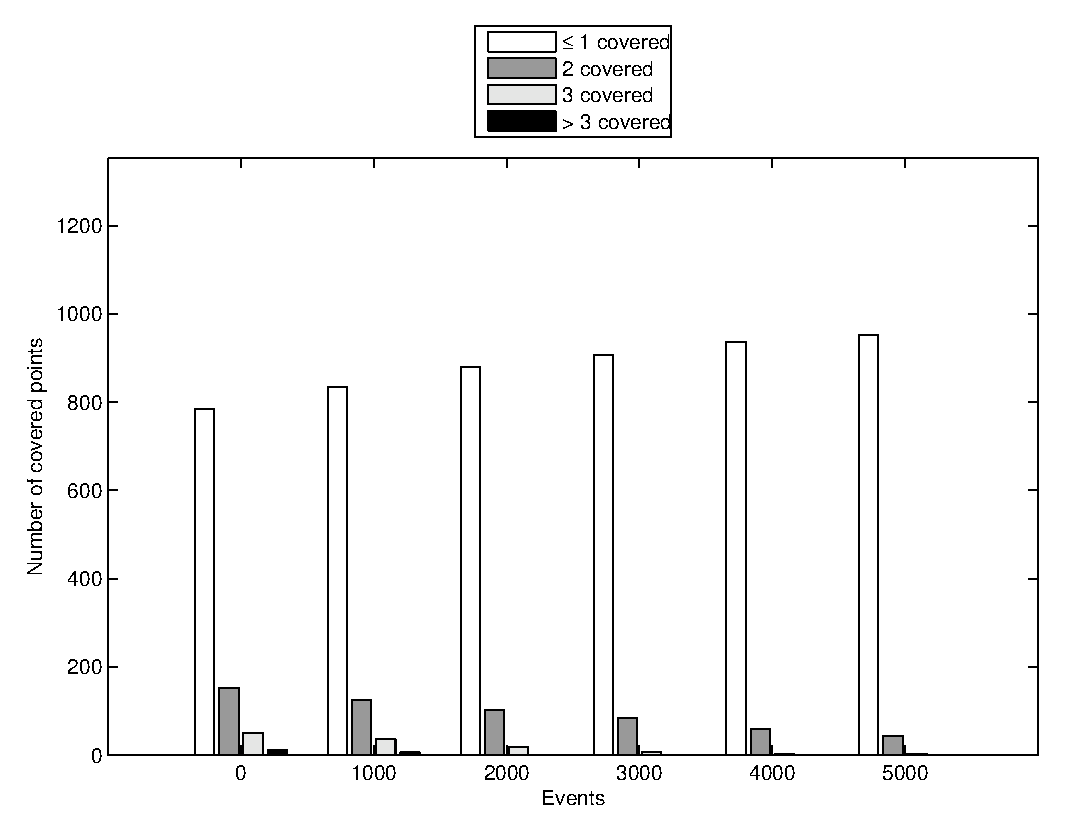
\includegraphics[width=0.48\textwidth]{experiments/4000nodes/1.norechargeVSrecharge/coverage_leach.eps}}
  \subfloat[Leach με Φορτιστή]{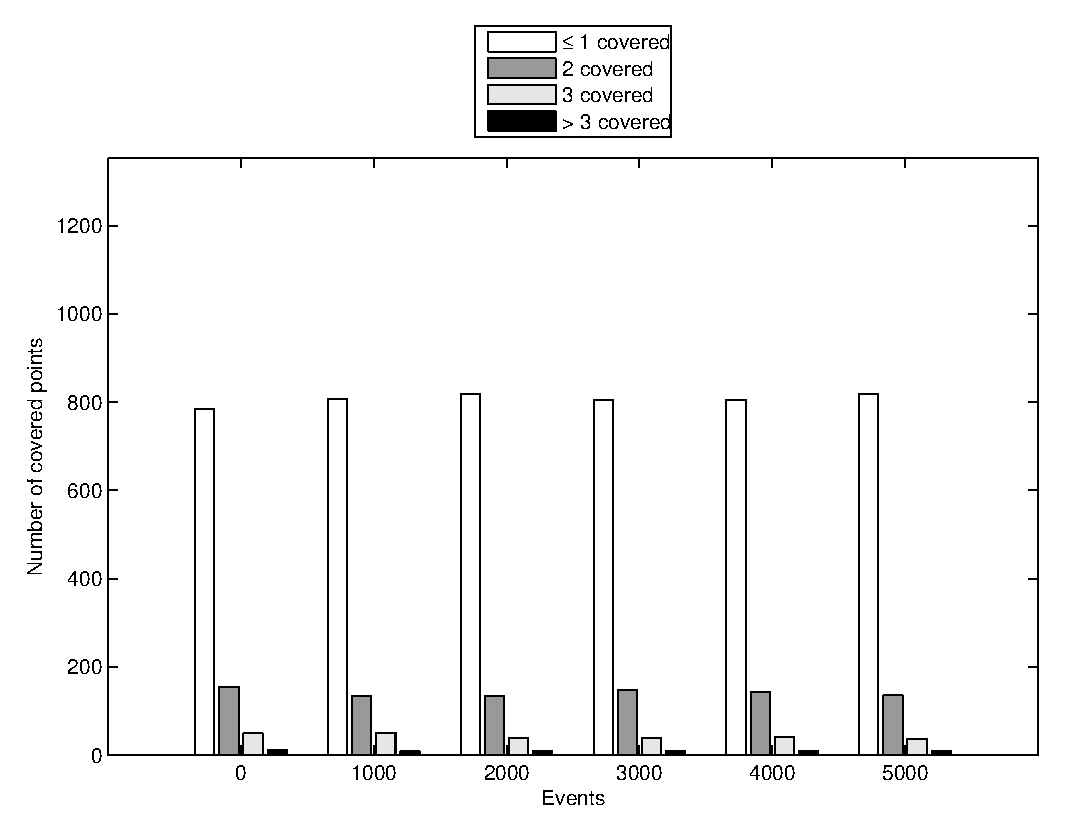
\includegraphics[width=0.48\textwidth]{experiments/4000nodes/1.norechargeVSrecharge/coverage_leach_rc.eps}}
  \caption{Κάλυψη του δικτύου κατα την πάροδο του χρόνου για το πρωτόκολλο Leach. Συγκρίνοντας τις 2 γραφικές παραστάσεις φαίνεται οτι στο δίκτυο με φορτιστή
υπάρχει καλύτερη κάλυψη των σημείων του δικτύου.}
  \label{fig:5_1exp_3_2}
\end{figure}

\begin{figure}[H]
  \centering
  \subfloat[$\text{E}_{i}$]{\includegraphics[width=0.48\textwidth]{experiments/4000nodes/1.norechargeVSrecharge/coverage_ei.eps}}
  \subfloat[$\text{E}_{i}$ με Φορτιστή]{\includegraphics[width=0.48\textwidth]{experiments/4000nodes/1.norechargeVSrecharge/coverage_ei_rc.eps}}
  \caption{Κάλυψη του δικτύου κατα την πάροδο του χρόνου για το πρωτόκολλο $\text{E}_{i}$. Συγκρίνοντας τις 2 γραφικές παραστάσεις φαίνεται οτι στο δίκτυο με φορτιστή
υπάρχει καλύτερη κάλυψη των σημείων του δικτύου.}
  \label{fig:5_1exp_3_3}
\end{figure}




%%%%%%%%%%%%%%%%%%%%%%%%%%%% 4. ENERGY MAPS %%%%%%%%%%%%%%%%%%%%%%%%%%%%%%%%%%%%%

\begin{figure}[H]
  \centering
  \subfloat[Greedy]{\includegraphics[width=0.48\textwidth]{experiments/4000nodes/1.norechargeVSrecharge/energy_greedy.eps}}
  \subfloat[Greedy με Φορτιστή]{\includegraphics[width=0.48\textwidth]{experiments/4000nodes/1.norechargeVSrecharge/energy_greedy_rc.eps}}
  \caption{Ενεργιακός χάρτης του δικτύου κατα την πάροδο του χρόνου για το πρωτόκολλο Greedy. Όσο πιο μαύρο τόσο λιγότερη ενέργεια έχει ο κόμβος. Συγκρίνοντας τις 2
γραφικές παραστάσεις φαίνεται οτι στο δίκτυο με φορτιστή υπάρχει καλύτερη εξισορρόπηση ενέργειας.}
  \label{fig:5_1exp_4_1}
\end{figure}

\begin{figure}[H]
  \centering
  \subfloat[Leach]{\includegraphics[width=0.48\textwidth]{experiments/4000nodes/1.norechargeVSrecharge/energy_leach.eps}}
  \subfloat[Leach με Φορτιστή]{\includegraphics[width=0.48\textwidth]{experiments/4000nodes/1.norechargeVSrecharge/energy_leach_rc.eps}}
  \caption{Κάλυψη του δικτύου κατα την πάροδο του χρόνου για το πρωτόκολλο Leach. Όσο πιο μαύρο τόσο λιγότερη ενέργεια έχει ο κόμβος. Συγκρίνοντας τις 2 γραφικές
παραστάσεις φαίνεται οτι στο δίκτυο με φορτιστή υπάρχει καλύτερη εξισορρόπηση ενέργειας.}
  \label{fig:5_1exp_4_2}
\end{figure}

\begin{figure}[H]
  \centering
  \subfloat[$\text{E}_{i}$]{\includegraphics[width=0.48\textwidth]{experiments/4000nodes/1.norechargeVSrecharge/energy_ei.eps}}
  \subfloat[$\text{E}_{i}$ με Φορτιστή]{\includegraphics[width=0.48\textwidth]{experiments/4000nodes/1.norechargeVSrecharge/energy_ei_rc.eps}}
  \caption{Κάλυψη του δικτύου κατα την πάροδο του χρόνου για το πρωτόκολλο $\text{E}_{i}$. Όσο πιο μαύρο τόσο λιγότερη ενέργεια έχει ο κόμβος. Συγκρίνοντας τις 2
γραφικές παραστάσεις φαίνεται οτι στο δίκτυο με φορτιστή υπάρχει καλύτερη εξισορρόπηση ενέργειας.}
  \label{fig:5_1exp_4_3}
\end{figure}



\subsection{Ολική και Μερική Φόρτιση}\label{subc:result5_2}
%%%%%%%%%%%%%%%%%%%%%%%%%%%% 1. LIFETIME %%%%%%%%%%%%%%%%%%%%%%%%%%%%%%%%%%%%%
\begin{figure}[H]
  \centering
  \subfloat[Greedy]{\includegraphics[width=0.32\textwidth]{experiments/4000nodes/2.partialVSfull/alive_nodes_greedy_rc_full-per.eps}}
  \subfloat[Leach]{\includegraphics[width=0.32\textwidth]{experiments/4000nodes/2.partialVSfull/alive_nodes_leach_rc_full-per.eps}}
  \subfloat[$\text{E}_{i}$]{\includegraphics[width=0.32\textwidth]{experiments/4000nodes/2.partialVSfull/alive_nodes_ei_rc_full-per.eps}}
  \caption{Ζωντανοί κόμβοι κατά την πάροδο του χρόνου. Η συνεχόμενη γραμμή αντιστοιχεί στην μερική φόρτιση. Στο Greedy πρωτόκολλο, η πλήρης φόρτιση έχει
ελάχιστα καλύτερα αποτελέσματα και έρχεται σε αντιστοίχιση με την εικόνα \ref{fig:2exp_1_1}. Αυτό συμβαίνει γιατί ο ρυθμός κατανάλωσης των κόμβων που είναι κοντά
στην Πηγή είναι πολύ μεγάλος και επομένως συμφέρει να φορτίζονται πλήρως. Αντίθετα στα άλλα 2 πρωτόκολλα, η μερική φόρτιση υπερτερεί της στρατηγικής της πλήρους
φόρτισης αλλά χωρίς μεγάλη διαφορά όπως στην περίπτωση των 1000 κόμβων.}
  \label{fig:5_2exp_1_1}
\end{figure}

%%%%%%%%%%%%%%%%%%%%%%%%%%%% 3. COVERAGE %%%%%%%%%%%%%%%%%%%%%%%%%%%%%%%%%%%%%
\begin{figure}[H]
  \centering
  \subfloat[Greedy με ολική Φόρτιση]{\includegraphics[width=0.48\textwidth]{experiments/4000nodes/2.partialVSfull/coverage_greedy_rc_full.eps}}
  \subfloat[Greedy με μερική Φόρτιση]{\includegraphics[width=0.48\textwidth]{experiments/4000nodes/2.partialVSfull/coverage_greedy_rc_per.eps}}
  \caption{Κάλυψη του δικτύου κατα την πάροδο του χρόνου για το πρωτόκολλο Greedy. Οι δύο στρατηγικές έχουν παρόμοια αποτελέσματα. Αυτό
συμβαίνει γιατί ο ρυθμός κατανάλωσης των κόμβων που είναι κοντά στην Πηγή είναι πολύ μεγάλος και επομένως η στρατηγική της μερικής φόρτισης δεν αποδίδει καλά.}
  \label{fig:5_2exp_3_1}
\end{figure}

\begin{figure}[H]
  \centering
  \subfloat[Leach με ολική Φόρτιση]{\includegraphics[width=0.48\textwidth]{experiments/4000nodes/2.partialVSfull/coverage_leach_rc_full.eps}}
  \subfloat[Leach με μερική Φόρτιση]{\includegraphics[width=0.48\textwidth]{experiments/4000nodes/2.partialVSfull/coverage_leach_rc_per.eps}}
  \caption{Κάλυψη του δικτύου κατα την πάροδο του χρόνου για το πρωτόκολλο Leach. Δεν είναι εμφανές ποια στρατηγική έχει καλύτερα λόγω του μεγάλου αριθμού κόμβων.}
  \label{fig:5_2exp_3_2}
\end{figure}

\begin{figure}[H]
  \centering
  \subfloat[$\text{E}_{i}$ με ολική Φόρτιση]{\includegraphics[width=0.48\textwidth]{experiments/4000nodes/2.partialVSfull/coverage_ei_rc_full.eps}}
  \subfloat[$\text{E}_{i}$ με μερική Φόρτιση]{\includegraphics[width=0.48\textwidth]{experiments/4000nodes/2.partialVSfull/coverage_ei_rc_per.eps}}
  \caption{Κάλυψη του δικτύου κατα την πάροδο του χρόνου για το πρωτόκολλο $\text{E}_{i}$. Δεν είναι εμφανές ποια στρατηγική έχει καλύτερα λόγω του μεγάλου αριθμού
κόμβων.}
  \label{fig:5_2exp_3_3}
\end{figure}


\subsection{Ποσοστό Ενέργειας στον Φορτιστή}\label{subc:result5_3}
%%%%%%%%%%%%%%%%%%%%%%%%%%%% 1. LIFETIME %%%%%%%%%%%%%%%%%%%%%%%%%%%%%%%%%%%%%
\begin{figure}[H]
  \centering
  \includegraphics[width=0.85\textwidth]{experiments/4000nodes/3.smallVSbigpercentage/alive_nodes_greedy_rc_per_our.eps}
  \caption{Ζωντανοί κόμβοι κατά την πάροδο του χρόνου στο Greedy πρωτόκολλο με ποικίλα ποσοστά ενέργειας στον κινητό φορτιστή. Στη γραφική αυτή φαίνεται ξεκάθαρα η
ανικανότητα του κινητού φορτιστή να διαχειριστεί αποδοτικά μεγάλο μέρος της συνολικής ενέργειας του δικτύου λόγω μεγάλου αριθμού κόμβων.}
  \label{fig:5_3exp_1_1}
\end{figure}

\begin{figure}[H]
  \centering
   \includegraphics[width=0.85\textwidth]{experiments/4000nodes/3.smallVSbigpercentage/alive_nodes_leach_rc_per_our.eps}
  \caption{Ζωντανοί κόμβοι κατά την πάροδο του χρόνου στο Leach πρωτόκολλο με ποικίλα ποσοστά ενέργειας στον κινητό φορτιστή. Στη γραφική αυτή φαίνεται ξεκάθαρα η
ανικανότητα του κινητού φορτιστή να διαχειριστεί αποδοτικά μεγάλο μέρος της συνολικής ενέργειας του δικτύου λόγω μεγάλου αριθμού κόμβων.}
  \label{fig:5_3exp_1_2}
\end{figure}

\begin{figure}[H]
  \centering
   \includegraphics[width=0.85\textwidth]{experiments/4000nodes/3.smallVSbigpercentage/alive_nodes_ei_rc_per_our.eps}
  \caption{Ζωντανοί κόμβοι κατά την πάροδο του χρόνου στο $\text{E}_{i}$ πρωτόκολλο με ποικίλα ποσοστά ενέργειας στον κινητό φορτιστή. Στη γραφική αυτή φαίνεται
ξεκάθαρα η ανικανότητα του κινητού φορτιστή να διαχειριστεί αποδοτικά μεγάλο μέρος της συνολικής ενέργειας του δικτύου λόγω μεγάλου αριθμού κόμβων.}
  \label{fig:5_3exp_1_3}
\end{figure}

\subsection{Σύγκριση Διαδρομών Φορτιστή}\label{subc:result5_4}
%%%%%%%%%%%%%%%%%%%%%%%%%%%% 1. LIFETIME %%%%%%%%%%%%%%%%%%%%%%%%%%%%%%%%%%%%%
\begin{figure}[H]
  \centering
  \includegraphics[width=0.9\textwidth]{experiments/4000nodes/4.ourVSnaive/alive_nodes_greedy_rc_per_our-spiral-random-diameter-heuristic.eps}
  \caption{Ζωντανοί κόμβοι κατά την πάροδο του χρόνου στο Greedy πρωτόκολλο για τις διάφορες διαδρομές του κινητού φορτιστή. Χρησιμοποιείται μερική φόρτιση και έχει
δωθεί το 20\% της ενέργειας στον φορτιστή.}
  \label{fig:5_4exp_1_1}
\end{figure}

\begin{figure}[H]
  \centering
  \includegraphics[width=0.9\textwidth]{experiments/4000nodes/4.ourVSnaive/alive_nodes_leach_rc_per_our-spiral-random-diameter-heuristic.eps}
  \caption{Ζωντανοί κόμβοι κατά την πάροδο του χρόνου στο Leach πρωτόκολλο για τις διάφορες διαδρομές του κινητού φορτιστή. Χρησιμοποιείται μερική φόρτιση και έχει
δωθεί το 20\% της ενέργειας στον φορτιστή.}
  \label{fig:5_4exp_1_2}
\end{figure}

\begin{figure}[H]
  \centering
  \includegraphics[width=0.9\textwidth]{experiments/4000nodes/4.ourVSnaive/alive_nodes_ei_rc_per_our-spiral-random-diameter-heuristic.eps}
  \caption{Ζωντανοί κόμβοι κατά την πάροδο του χρόνου στο $\text{E}_{i}$ πρωτόκολλο για τις διάφορες διαδρομές του κινητού φορτιστή. Χρησιμοποιείται μερική φόρτιση
και έχει δωθεί το 20\% της ενέργειας στον φορτιστή.}
  \label{fig:5_4exp_1_3}
\end{figure}


\section{Παραμετροποιώντας την Τεχνολογία Φόρτισης}\label{sc:result6}

%%%%%%%%%%%%%%%%%%%%%%%%%%%% 1. LIFETIME %%%%%%%%%%%%%%%%%%%%%%%%%%%%%%%%%%%%%
\begin{figure}[H]
  \centering
  \includegraphics[width=0.85\textwidth]{experiments/4000nodes/3.smallVSbigpercentage/alive_nodes_greedy_rc_per_our.eps}
  \caption{Ζωντανοί κόμβοι κατά την πάροδο του χρόνου στο Greedy πρωτόκολλο με ποικίλα ποσοστά ενέργειας στον κινητό φορτιστή. Στη γραφική αυτή φαίνεται ξεκάθαρα η
ανικανότητα του κινητού φορτιστή να διαχειριστεί αποδοτικά μεγάλο μέρος της συνολικής ενέργειας του δικτύου λόγω μεγάλου αριθμού κόμβων.}
  \label{fig:5_3exp_1_1}
\end{figure}

\begin{figure}[H]
  \centering
   \includegraphics[width=0.85\textwidth]{experiments/4000nodes/3.smallVSbigpercentage/alive_nodes_leach_rc_per_our.eps}
  \caption{Ζωντανοί κόμβοι κατά την πάροδο του χρόνου στο Leach πρωτόκολλο με ποικίλα ποσοστά ενέργειας στον κινητό φορτιστή. Στη γραφική αυτή φαίνεται ξεκάθαρα η
ανικανότητα του κινητού φορτιστή να διαχειριστεί αποδοτικά μεγάλο μέρος της συνολικής ενέργειας του δικτύου λόγω μεγάλου αριθμού κόμβων.}
  \label{fig:5_3exp_1_2}
\end{figure}

\begin{figure}[H]
  \centering
   \includegraphics[width=0.85\textwidth]{experiments/4000nodes/3.smallVSbigpercentage/alive_nodes_ei_rc_per_our.eps}
  \caption{Ζωντανοί κόμβοι κατά την πάροδο του χρόνου στο $\text{E}_{i}$ πρωτόκολλο με ποικίλα ποσοστά ενέργειας στον κινητό φορτιστή. Στη γραφική αυτή φαίνεται
ξεκάθαρα η ανικανότητα του κινητού φορτιστή να διαχειριστεί αποδοτικά μεγάλο μέρος της συνολικής ενέργειας του δικτύου λόγω μεγάλου αριθμού κόμβων.}
  \label{fig:5_3exp_1_3}
\end{figure}